
% Default to the notebook output style

    


% Inherit from the specified cell style.




    
\documentclass[11pt]{article}

    
    
    \usepackage[T1]{fontenc}
    % Nicer default font (+ math font) than Computer Modern for most use cases
    \usepackage{mathpazo}

    % Basic figure setup, for now with no caption control since it's done
    % automatically by Pandoc (which extracts ![](path) syntax from Markdown).
    \usepackage{graphicx}
    % We will generate all images so they have a width \maxwidth. This means
    % that they will get their normal width if they fit onto the page, but
    % are scaled down if they would overflow the margins.
    \makeatletter
    \def\maxwidth{\ifdim\Gin@nat@width>\linewidth\linewidth
    \else\Gin@nat@width\fi}
    \makeatother
    \let\Oldincludegraphics\includegraphics
    % Set max figure width to be 80% of text width, for now hardcoded.
    \renewcommand{\includegraphics}[1]{\Oldincludegraphics[width=.8\maxwidth]{#1}}
    % Ensure that by default, figures have no caption (until we provide a
    % proper Figure object with a Caption API and a way to capture that
    % in the conversion process - todo).
    \usepackage{caption}
    \DeclareCaptionLabelFormat{nolabel}{}
    \captionsetup{labelformat=nolabel}

    \usepackage{adjustbox} % Used to constrain images to a maximum size 
    \usepackage{xcolor} % Allow colors to be defined
    \usepackage{enumerate} % Needed for markdown enumerations to work
    \usepackage{geometry} % Used to adjust the document margins
    \usepackage{amsmath} % Equations
    \usepackage{amssymb} % Equations
    \usepackage{textcomp} % defines textquotesingle
    % Hack from http://tex.stackexchange.com/a/47451/13684:
    \AtBeginDocument{%
        \def\PYZsq{\textquotesingle}% Upright quotes in Pygmentized code
    }
    \usepackage{upquote} % Upright quotes for verbatim code
    \usepackage{eurosym} % defines \euro
    \usepackage[mathletters]{ucs} % Extended unicode (utf-8) support
    \usepackage[utf8x]{inputenc} % Allow utf-8 characters in the tex document
    \usepackage{fancyvrb} % verbatim replacement that allows latex
    \usepackage{grffile} % extends the file name processing of package graphics 
                         % to support a larger range 
    % The hyperref package gives us a pdf with properly built
    % internal navigation ('pdf bookmarks' for the table of contents,
    % internal cross-reference links, web links for URLs, etc.)
    \usepackage{hyperref}
    \usepackage{longtable} % longtable support required by pandoc >1.10
    \usepackage{booktabs}  % table support for pandoc > 1.12.2
    \usepackage[inline]{enumitem} % IRkernel/repr support (it uses the enumerate* environment)
    \usepackage[normalem]{ulem} % ulem is needed to support strikethroughs (\sout)
                                % normalem makes italics be italics, not underlines
    

    
    
    % Colors for the hyperref package
    \definecolor{urlcolor}{rgb}{0,.145,.698}
    \definecolor{linkcolor}{rgb}{.71,0.21,0.01}
    \definecolor{citecolor}{rgb}{.12,.54,.11}

    % ANSI colors
    \definecolor{ansi-black}{HTML}{3E424D}
    \definecolor{ansi-black-intense}{HTML}{282C36}
    \definecolor{ansi-red}{HTML}{E75C58}
    \definecolor{ansi-red-intense}{HTML}{B22B31}
    \definecolor{ansi-green}{HTML}{00A250}
    \definecolor{ansi-green-intense}{HTML}{007427}
    \definecolor{ansi-yellow}{HTML}{DDB62B}
    \definecolor{ansi-yellow-intense}{HTML}{B27D12}
    \definecolor{ansi-blue}{HTML}{208FFB}
    \definecolor{ansi-blue-intense}{HTML}{0065CA}
    \definecolor{ansi-magenta}{HTML}{D160C4}
    \definecolor{ansi-magenta-intense}{HTML}{A03196}
    \definecolor{ansi-cyan}{HTML}{60C6C8}
    \definecolor{ansi-cyan-intense}{HTML}{258F8F}
    \definecolor{ansi-white}{HTML}{C5C1B4}
    \definecolor{ansi-white-intense}{HTML}{A1A6B2}

    % commands and environments needed by pandoc snippets
    % extracted from the output of `pandoc -s`
    \providecommand{\tightlist}{%
      \setlength{\itemsep}{0pt}\setlength{\parskip}{0pt}}
    \DefineVerbatimEnvironment{Highlighting}{Verbatim}{commandchars=\\\{\}}
    % Add ',fontsize=\small' for more characters per line
    \newenvironment{Shaded}{}{}
    \newcommand{\KeywordTok}[1]{\textcolor[rgb]{0.00,0.44,0.13}{\textbf{{#1}}}}
    \newcommand{\DataTypeTok}[1]{\textcolor[rgb]{0.56,0.13,0.00}{{#1}}}
    \newcommand{\DecValTok}[1]{\textcolor[rgb]{0.25,0.63,0.44}{{#1}}}
    \newcommand{\BaseNTok}[1]{\textcolor[rgb]{0.25,0.63,0.44}{{#1}}}
    \newcommand{\FloatTok}[1]{\textcolor[rgb]{0.25,0.63,0.44}{{#1}}}
    \newcommand{\CharTok}[1]{\textcolor[rgb]{0.25,0.44,0.63}{{#1}}}
    \newcommand{\StringTok}[1]{\textcolor[rgb]{0.25,0.44,0.63}{{#1}}}
    \newcommand{\CommentTok}[1]{\textcolor[rgb]{0.38,0.63,0.69}{\textit{{#1}}}}
    \newcommand{\OtherTok}[1]{\textcolor[rgb]{0.00,0.44,0.13}{{#1}}}
    \newcommand{\AlertTok}[1]{\textcolor[rgb]{1.00,0.00,0.00}{\textbf{{#1}}}}
    \newcommand{\FunctionTok}[1]{\textcolor[rgb]{0.02,0.16,0.49}{{#1}}}
    \newcommand{\RegionMarkerTok}[1]{{#1}}
    \newcommand{\ErrorTok}[1]{\textcolor[rgb]{1.00,0.00,0.00}{\textbf{{#1}}}}
    \newcommand{\NormalTok}[1]{{#1}}
    
    % Additional commands for more recent versions of Pandoc
    \newcommand{\ConstantTok}[1]{\textcolor[rgb]{0.53,0.00,0.00}{{#1}}}
    \newcommand{\SpecialCharTok}[1]{\textcolor[rgb]{0.25,0.44,0.63}{{#1}}}
    \newcommand{\VerbatimStringTok}[1]{\textcolor[rgb]{0.25,0.44,0.63}{{#1}}}
    \newcommand{\SpecialStringTok}[1]{\textcolor[rgb]{0.73,0.40,0.53}{{#1}}}
    \newcommand{\ImportTok}[1]{{#1}}
    \newcommand{\DocumentationTok}[1]{\textcolor[rgb]{0.73,0.13,0.13}{\textit{{#1}}}}
    \newcommand{\AnnotationTok}[1]{\textcolor[rgb]{0.38,0.63,0.69}{\textbf{\textit{{#1}}}}}
    \newcommand{\CommentVarTok}[1]{\textcolor[rgb]{0.38,0.63,0.69}{\textbf{\textit{{#1}}}}}
    \newcommand{\VariableTok}[1]{\textcolor[rgb]{0.10,0.09,0.49}{{#1}}}
    \newcommand{\ControlFlowTok}[1]{\textcolor[rgb]{0.00,0.44,0.13}{\textbf{{#1}}}}
    \newcommand{\OperatorTok}[1]{\textcolor[rgb]{0.40,0.40,0.40}{{#1}}}
    \newcommand{\BuiltInTok}[1]{{#1}}
    \newcommand{\ExtensionTok}[1]{{#1}}
    \newcommand{\PreprocessorTok}[1]{\textcolor[rgb]{0.74,0.48,0.00}{{#1}}}
    \newcommand{\AttributeTok}[1]{\textcolor[rgb]{0.49,0.56,0.16}{{#1}}}
    \newcommand{\InformationTok}[1]{\textcolor[rgb]{0.38,0.63,0.69}{\textbf{\textit{{#1}}}}}
    \newcommand{\WarningTok}[1]{\textcolor[rgb]{0.38,0.63,0.69}{\textbf{\textit{{#1}}}}}
    
    
    % Define a nice break command that doesn't care if a line doesn't already
    % exist.
    \def\br{\hspace*{\fill} \\* }
    % Math Jax compatability definitions
    \def\gt{>}
    \def\lt{<}
    % Document parameters
    \title{BurstPy-v1.2-Walkthrough}
    
    
    

    % Pygments definitions
    
\makeatletter
\def\PY@reset{\let\PY@it=\relax \let\PY@bf=\relax%
    \let\PY@ul=\relax \let\PY@tc=\relax%
    \let\PY@bc=\relax \let\PY@ff=\relax}
\def\PY@tok#1{\csname PY@tok@#1\endcsname}
\def\PY@toks#1+{\ifx\relax#1\empty\else%
    \PY@tok{#1}\expandafter\PY@toks\fi}
\def\PY@do#1{\PY@bc{\PY@tc{\PY@ul{%
    \PY@it{\PY@bf{\PY@ff{#1}}}}}}}
\def\PY#1#2{\PY@reset\PY@toks#1+\relax+\PY@do{#2}}

\expandafter\def\csname PY@tok@w\endcsname{\def\PY@tc##1{\textcolor[rgb]{0.73,0.73,0.73}{##1}}}
\expandafter\def\csname PY@tok@c\endcsname{\let\PY@it=\textit\def\PY@tc##1{\textcolor[rgb]{0.25,0.50,0.50}{##1}}}
\expandafter\def\csname PY@tok@cp\endcsname{\def\PY@tc##1{\textcolor[rgb]{0.74,0.48,0.00}{##1}}}
\expandafter\def\csname PY@tok@k\endcsname{\let\PY@bf=\textbf\def\PY@tc##1{\textcolor[rgb]{0.00,0.50,0.00}{##1}}}
\expandafter\def\csname PY@tok@kp\endcsname{\def\PY@tc##1{\textcolor[rgb]{0.00,0.50,0.00}{##1}}}
\expandafter\def\csname PY@tok@kt\endcsname{\def\PY@tc##1{\textcolor[rgb]{0.69,0.00,0.25}{##1}}}
\expandafter\def\csname PY@tok@o\endcsname{\def\PY@tc##1{\textcolor[rgb]{0.40,0.40,0.40}{##1}}}
\expandafter\def\csname PY@tok@ow\endcsname{\let\PY@bf=\textbf\def\PY@tc##1{\textcolor[rgb]{0.67,0.13,1.00}{##1}}}
\expandafter\def\csname PY@tok@nb\endcsname{\def\PY@tc##1{\textcolor[rgb]{0.00,0.50,0.00}{##1}}}
\expandafter\def\csname PY@tok@nf\endcsname{\def\PY@tc##1{\textcolor[rgb]{0.00,0.00,1.00}{##1}}}
\expandafter\def\csname PY@tok@nc\endcsname{\let\PY@bf=\textbf\def\PY@tc##1{\textcolor[rgb]{0.00,0.00,1.00}{##1}}}
\expandafter\def\csname PY@tok@nn\endcsname{\let\PY@bf=\textbf\def\PY@tc##1{\textcolor[rgb]{0.00,0.00,1.00}{##1}}}
\expandafter\def\csname PY@tok@ne\endcsname{\let\PY@bf=\textbf\def\PY@tc##1{\textcolor[rgb]{0.82,0.25,0.23}{##1}}}
\expandafter\def\csname PY@tok@nv\endcsname{\def\PY@tc##1{\textcolor[rgb]{0.10,0.09,0.49}{##1}}}
\expandafter\def\csname PY@tok@no\endcsname{\def\PY@tc##1{\textcolor[rgb]{0.53,0.00,0.00}{##1}}}
\expandafter\def\csname PY@tok@nl\endcsname{\def\PY@tc##1{\textcolor[rgb]{0.63,0.63,0.00}{##1}}}
\expandafter\def\csname PY@tok@ni\endcsname{\let\PY@bf=\textbf\def\PY@tc##1{\textcolor[rgb]{0.60,0.60,0.60}{##1}}}
\expandafter\def\csname PY@tok@na\endcsname{\def\PY@tc##1{\textcolor[rgb]{0.49,0.56,0.16}{##1}}}
\expandafter\def\csname PY@tok@nt\endcsname{\let\PY@bf=\textbf\def\PY@tc##1{\textcolor[rgb]{0.00,0.50,0.00}{##1}}}
\expandafter\def\csname PY@tok@nd\endcsname{\def\PY@tc##1{\textcolor[rgb]{0.67,0.13,1.00}{##1}}}
\expandafter\def\csname PY@tok@s\endcsname{\def\PY@tc##1{\textcolor[rgb]{0.73,0.13,0.13}{##1}}}
\expandafter\def\csname PY@tok@sd\endcsname{\let\PY@it=\textit\def\PY@tc##1{\textcolor[rgb]{0.73,0.13,0.13}{##1}}}
\expandafter\def\csname PY@tok@si\endcsname{\let\PY@bf=\textbf\def\PY@tc##1{\textcolor[rgb]{0.73,0.40,0.53}{##1}}}
\expandafter\def\csname PY@tok@se\endcsname{\let\PY@bf=\textbf\def\PY@tc##1{\textcolor[rgb]{0.73,0.40,0.13}{##1}}}
\expandafter\def\csname PY@tok@sr\endcsname{\def\PY@tc##1{\textcolor[rgb]{0.73,0.40,0.53}{##1}}}
\expandafter\def\csname PY@tok@ss\endcsname{\def\PY@tc##1{\textcolor[rgb]{0.10,0.09,0.49}{##1}}}
\expandafter\def\csname PY@tok@sx\endcsname{\def\PY@tc##1{\textcolor[rgb]{0.00,0.50,0.00}{##1}}}
\expandafter\def\csname PY@tok@m\endcsname{\def\PY@tc##1{\textcolor[rgb]{0.40,0.40,0.40}{##1}}}
\expandafter\def\csname PY@tok@gh\endcsname{\let\PY@bf=\textbf\def\PY@tc##1{\textcolor[rgb]{0.00,0.00,0.50}{##1}}}
\expandafter\def\csname PY@tok@gu\endcsname{\let\PY@bf=\textbf\def\PY@tc##1{\textcolor[rgb]{0.50,0.00,0.50}{##1}}}
\expandafter\def\csname PY@tok@gd\endcsname{\def\PY@tc##1{\textcolor[rgb]{0.63,0.00,0.00}{##1}}}
\expandafter\def\csname PY@tok@gi\endcsname{\def\PY@tc##1{\textcolor[rgb]{0.00,0.63,0.00}{##1}}}
\expandafter\def\csname PY@tok@gr\endcsname{\def\PY@tc##1{\textcolor[rgb]{1.00,0.00,0.00}{##1}}}
\expandafter\def\csname PY@tok@ge\endcsname{\let\PY@it=\textit}
\expandafter\def\csname PY@tok@gs\endcsname{\let\PY@bf=\textbf}
\expandafter\def\csname PY@tok@gp\endcsname{\let\PY@bf=\textbf\def\PY@tc##1{\textcolor[rgb]{0.00,0.00,0.50}{##1}}}
\expandafter\def\csname PY@tok@go\endcsname{\def\PY@tc##1{\textcolor[rgb]{0.53,0.53,0.53}{##1}}}
\expandafter\def\csname PY@tok@gt\endcsname{\def\PY@tc##1{\textcolor[rgb]{0.00,0.27,0.87}{##1}}}
\expandafter\def\csname PY@tok@err\endcsname{\def\PY@bc##1{\setlength{\fboxsep}{0pt}\fcolorbox[rgb]{1.00,0.00,0.00}{1,1,1}{\strut ##1}}}
\expandafter\def\csname PY@tok@kc\endcsname{\let\PY@bf=\textbf\def\PY@tc##1{\textcolor[rgb]{0.00,0.50,0.00}{##1}}}
\expandafter\def\csname PY@tok@kd\endcsname{\let\PY@bf=\textbf\def\PY@tc##1{\textcolor[rgb]{0.00,0.50,0.00}{##1}}}
\expandafter\def\csname PY@tok@kn\endcsname{\let\PY@bf=\textbf\def\PY@tc##1{\textcolor[rgb]{0.00,0.50,0.00}{##1}}}
\expandafter\def\csname PY@tok@kr\endcsname{\let\PY@bf=\textbf\def\PY@tc##1{\textcolor[rgb]{0.00,0.50,0.00}{##1}}}
\expandafter\def\csname PY@tok@bp\endcsname{\def\PY@tc##1{\textcolor[rgb]{0.00,0.50,0.00}{##1}}}
\expandafter\def\csname PY@tok@fm\endcsname{\def\PY@tc##1{\textcolor[rgb]{0.00,0.00,1.00}{##1}}}
\expandafter\def\csname PY@tok@vc\endcsname{\def\PY@tc##1{\textcolor[rgb]{0.10,0.09,0.49}{##1}}}
\expandafter\def\csname PY@tok@vg\endcsname{\def\PY@tc##1{\textcolor[rgb]{0.10,0.09,0.49}{##1}}}
\expandafter\def\csname PY@tok@vi\endcsname{\def\PY@tc##1{\textcolor[rgb]{0.10,0.09,0.49}{##1}}}
\expandafter\def\csname PY@tok@vm\endcsname{\def\PY@tc##1{\textcolor[rgb]{0.10,0.09,0.49}{##1}}}
\expandafter\def\csname PY@tok@sa\endcsname{\def\PY@tc##1{\textcolor[rgb]{0.73,0.13,0.13}{##1}}}
\expandafter\def\csname PY@tok@sb\endcsname{\def\PY@tc##1{\textcolor[rgb]{0.73,0.13,0.13}{##1}}}
\expandafter\def\csname PY@tok@sc\endcsname{\def\PY@tc##1{\textcolor[rgb]{0.73,0.13,0.13}{##1}}}
\expandafter\def\csname PY@tok@dl\endcsname{\def\PY@tc##1{\textcolor[rgb]{0.73,0.13,0.13}{##1}}}
\expandafter\def\csname PY@tok@s2\endcsname{\def\PY@tc##1{\textcolor[rgb]{0.73,0.13,0.13}{##1}}}
\expandafter\def\csname PY@tok@sh\endcsname{\def\PY@tc##1{\textcolor[rgb]{0.73,0.13,0.13}{##1}}}
\expandafter\def\csname PY@tok@s1\endcsname{\def\PY@tc##1{\textcolor[rgb]{0.73,0.13,0.13}{##1}}}
\expandafter\def\csname PY@tok@mb\endcsname{\def\PY@tc##1{\textcolor[rgb]{0.40,0.40,0.40}{##1}}}
\expandafter\def\csname PY@tok@mf\endcsname{\def\PY@tc##1{\textcolor[rgb]{0.40,0.40,0.40}{##1}}}
\expandafter\def\csname PY@tok@mh\endcsname{\def\PY@tc##1{\textcolor[rgb]{0.40,0.40,0.40}{##1}}}
\expandafter\def\csname PY@tok@mi\endcsname{\def\PY@tc##1{\textcolor[rgb]{0.40,0.40,0.40}{##1}}}
\expandafter\def\csname PY@tok@il\endcsname{\def\PY@tc##1{\textcolor[rgb]{0.40,0.40,0.40}{##1}}}
\expandafter\def\csname PY@tok@mo\endcsname{\def\PY@tc##1{\textcolor[rgb]{0.40,0.40,0.40}{##1}}}
\expandafter\def\csname PY@tok@ch\endcsname{\let\PY@it=\textit\def\PY@tc##1{\textcolor[rgb]{0.25,0.50,0.50}{##1}}}
\expandafter\def\csname PY@tok@cm\endcsname{\let\PY@it=\textit\def\PY@tc##1{\textcolor[rgb]{0.25,0.50,0.50}{##1}}}
\expandafter\def\csname PY@tok@cpf\endcsname{\let\PY@it=\textit\def\PY@tc##1{\textcolor[rgb]{0.25,0.50,0.50}{##1}}}
\expandafter\def\csname PY@tok@c1\endcsname{\let\PY@it=\textit\def\PY@tc##1{\textcolor[rgb]{0.25,0.50,0.50}{##1}}}
\expandafter\def\csname PY@tok@cs\endcsname{\let\PY@it=\textit\def\PY@tc##1{\textcolor[rgb]{0.25,0.50,0.50}{##1}}}

\def\PYZbs{\char`\\}
\def\PYZus{\char`\_}
\def\PYZob{\char`\{}
\def\PYZcb{\char`\}}
\def\PYZca{\char`\^}
\def\PYZam{\char`\&}
\def\PYZlt{\char`\<}
\def\PYZgt{\char`\>}
\def\PYZsh{\char`\#}
\def\PYZpc{\char`\%}
\def\PYZdl{\char`\$}
\def\PYZhy{\char`\-}
\def\PYZsq{\char`\'}
\def\PYZdq{\char`\"}
\def\PYZti{\char`\~}
% for compatibility with earlier versions
\def\PYZat{@}
\def\PYZlb{[}
\def\PYZrb{]}
\makeatother


    % Exact colors from NB
    \definecolor{incolor}{rgb}{0.0, 0.0, 0.5}
    \definecolor{outcolor}{rgb}{0.545, 0.0, 0.0}



    
    % Prevent overflowing lines due to hard-to-break entities
    \sloppy 
    % Setup hyperref package
    \hypersetup{
      breaklinks=true,  % so long urls are correctly broken across lines
      colorlinks=true,
      urlcolor=urlcolor,
      linkcolor=linkcolor,
      citecolor=citecolor,
      }
    % Slightly bigger margins than the latex defaults
    
    \geometry{verbose,tmargin=1in,bmargin=1in,lmargin=1in,rmargin=1in}
    
    

    \begin{document}
    
    
    \maketitle
    
    

    
    \section{BurstPy: a Quick
Walkthrough}\label{burstpy-a-quick-walkthrough}

This is a quick walkthrough of the autocorrelation statistical analysis
package I put together working for the Lagha Lab at IGMM in Montpellier,
France. \#\#\# What does it do? The purpose of this software package is
to quantify \emph{"bursty"} transcription dynamics in fly embryos. Due
to noise and stochastic (random) variability in GFP MS2 signal
cell-to-cell, an autocorrelation approach is necessary to decipher the
patterns by which gene promoters start and stop transcription. We rely
primarily on the derivation in Desponds et al (2016) for extracting
two-state promoter dynamics from data.

\subsubsection{What do I need to run
it?}\label{what-do-i-need-to-run-it}

The package runs on Python 3, and will (eventually) be implemented into
its own, standalone GUI interface for easy access within the lab
environment.

    \subsection{Why Autocorrelation?}\label{why-autocorrelation}

Recent advancements in gene splicing have made it possible to track
transcriptional processes (in \emph{drosophila} embryos) in real time.
The MS2 GFP cassette, a string of fluorescing molecules, can be attached
to an RNA Polymerase (polII) as it transcribes a section of a gene. The
result is a flourescent signal that can be tracked and measured over
time to illuminate how these polymerases behave during transcription.

Although the MS2 system is in itself a breakthrough, the resulting
signals or "traces" from each transcribing cell are inherently random
signals-\/-that is, they stem from a fundamentally \emph{stochastic}
process. What's more, measurement noise and cell-to-cell variability can
obscure dynamics even more, making it impossible to resolve single
traces by eye.

Signal autocorrelation is an approach that bypasses many of these
issues. Autocorrelation compares a random signal, \(X(t)\) with itself
at every time point, "sliding" the function along itself. Let's assume
for now that \(X(t)\) can either be "ON" or "OFF", each state for a
random duration of time. The autocorrelation function tells us to what
degree a signal "remembers" itself being either "ON" or "OFF". That is,
how similar is the signal at time \(t\), \(X(t) = X_t\), to itself at
time \(s\), when the signal \(X(t)\) = \(X_s\)?

The equation that describes this process is:

\begin{figure}
\centering
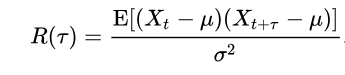
\includegraphics{tutorial/auto-eq.PNG}
\caption{auto-eq.PNG}
\end{figure}

where \(\mu\) is the mean of the signal, and \(\sigma^2\) is the
variance. A good illustration (courtesy of Wikipedia):

\begin{figure}
\centering
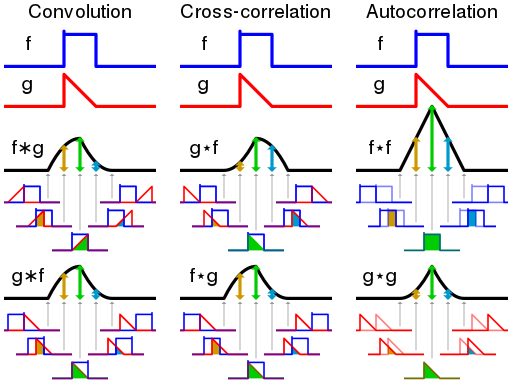
\includegraphics{tutorial/Comparison_convolution_correlation.png}
\caption{Comparison\_convolution\_correlation.png}
\end{figure}

Following some mathematical derivation (below), we find that the
autocorrelation function takes the form of an exponential decay curve,
dependent solely on the time \emph{delay} between comparison points in
the signal \(X(t)\).

The characteristic decay time, \(\tau_{char}\), can be linked to the
\emph{underlying random distribution} that tells \(X(t)\) how long to
stay "ON" or "OFF". In the case of Poisson-distributed wait durations,
\(\tau_{char}\) is the mean of the distribution.

    \subsection{Case Study: One-State Poisson Random
Promoter}\label{case-study-one-state-poisson-random-promoter}

\begin{figure}
\centering
\includegraphics{attachment:poisson-wait-time.png}
\caption{poisson-wait-time.png}
\end{figure}

When building our models of transcription, we assume that the trigger of
polymerase activity is a promoter state. This promoter state acts like a
switch: either the gene is "ON" or "OFF"-\/-e.g. our \(X(t)\) above.
Let's assume now that the promoter switches between 1 and -1 ("ON" and
"OFF") randomly, drawing each time between switches from a \emph{Poisson
distribution}. Poisson distributions are used to describe single,
uncorrelated events-\/-in this case, flipping the switch.

\[P(N(t) = n) = \frac{(\lambda t)^{n}e^{-\lambda t}}{n!} \]

Where \(\lambda\) is the mean of the distribution and \(N(t)\) is the
number of switches from ON to OFF. From here, the probability that
\(N(t)\) is even (\(X(t)=\) ON) at a given t is:

\[P((X(t) = 1 = ON)) = e^{-\lambda t}[1 + \frac{(\lambda t)^2}{2!} + \frac{(\lambda t)^4}{4!} + ...] \approx e^{-\lambda t}cosh(\lambda t)\]

Similarly, the probability that the switch lands in an OFF (N(t) is odd)
state is given as:

\[P((X(t) = -1 = OFF)) = e^{-\lambda t}[\lambda t + \frac{(\lambda t)^3}{3!} + \frac{(\lambda t)^5}{5!} + ...] \approx e^{-\lambda t}sinh(\lambda t)\]

    The discrete autocorrelation \(R(\tau)\) at lag \(\tau\) is:

\[ R_{yy}(\tau) = \sum_{n\in [-1, 1]}^{} {X(t)X(t+\tau)}\]

Where \(n\) can take on a value of \$\pm\$1. For a random process
governed by a probability distribution, the autocorrelation takes the
form:

\[ R_{yy}(\tau) = \sum_{j=0}^{1} {}\sum_{k=0}^{1} {x_k x_j P[X(t)=x_k]P[X(t+\tau) = x_j\mid X(t) = x_k]} \]

    The way this expression reads is that we compare the signal \(X(t)\) to
itself a short \(\tau\) time later, provided \(X(t) = x_k\) at \(t\).
Now, we know that our signal can take only values \$x\_i=\pm\$1. We also
know that \(P[X(t)=x_k]\), etc approximate the \(sinh\) and \(cosh\)
functions. Substituting these in allow us to solve \emph{analytically}
for the shape of \(R_{yy}\). Let's compare the signal at two different
times, \((t+\tau)=t_2)\) and \(t=t_1\)

    For \(x_k=1\), \(x_j=-1\) know that, if the signal at \(t_1\) and
\(t_2\) stays the same:

\[ P[X(t_2)=1|X(t_1)=1] = P[X(t_2)=-1\mid X(t_1)=-1] = e^{-\lambda (t_2 - t_1) }cosh(\lambda(t_2 - t_1))    \]

and if the signal changes, that

\[ P[X(t_2)=-1|X(t_1)=1] = P[X(t_2)=1\mid X(t_1)=-1] =  e^{-\lambda (t_2 - t_1) }sinh(\lambda(t_2 - t_1)) \]

    Then, plugging in everything into the expression for
\(R_{yy}(t_1, t_2)\), we obtain:

\[ R_{yy}(t_1, t_2) =  e^{-\lambda t_1}cosh(\lambda t_1) [e^{-\lambda (t_2 - t_1) }cosh(\lambda(t_2 - t_1)) - e^{-\lambda (t_2 - t_1) }sinh(\lambda(t_2 - t_1))] \]
\[- e^{-\lambda t_1}sinh(\lambda t_1) [e^{-\lambda (t_2 - t_1) }cosh(\lambda(t_2 - t_1)) - e^{-\lambda (t_2 - t_1) }sinh(\lambda(t_2 - t_1))]    \]

    This reduces (albeit with some algebra) to simply:

\[ R_{yy}(t_1, t_2) = e^{-\lambda (t_1-t_2)}\] or
\[ R_{yy}(\tau) = e^{-\lambda (\tau)} \]

So the autocorrelation function for a random telegraph (or binary
promoter) signal is simply an exponential decay function, dependent on
the time delay \(\tau = t_1 - t_2\) and the mean, \(\lambda\), of the
random (poisson) distribution. \(\lambda=1/\tau_{characteristic}\), so
fitting to the exponential curve we can determine the average time our
signal spends ON or OFF. We'll simulate this below to visualize the
solution:

    \begin{Verbatim}[commandchars=\\\{\}]
{\color{incolor}In [{\color{incolor}1}]:} \PY{k+kn}{import} \PY{n+nn}{numpy} \PY{k}{as} \PY{n+nn}{np}
        \PY{k+kn}{import} \PY{n+nn}{matplotlib}\PY{n+nn}{.}\PY{n+nn}{pyplot} \PY{k}{as} \PY{n+nn}{plt}
        
        \PY{c+c1}{\PYZsh{} Let\PYZsq{}s write a function to demonstrate our Poisson telegraph signal. Then we can change our inputs to see how a}
        \PY{c+c1}{\PYZsh{} numerical simulation can approach the analytic solution}
        \PY{k}{def} \PY{n+nf}{poisson\PYZus{}signal}\PY{p}{(}\PY{n}{sig\PYZus{}length}\PY{p}{,} \PY{n}{lmda}\PY{p}{)}\PY{p}{:}
            \PY{c+c1}{\PYZsh{} some input parameters for our signal and autocorrelation;}
            \PY{n}{lmda} \PY{o}{=} \PY{n}{lmda}  \PY{c+c1}{\PYZsh{} average duration (\PYZsq{}seconds\PYZsq{})}
            \PY{n}{sig\PYZus{}length} \PY{o}{=} \PY{n}{sig\PYZus{}length}       \PY{c+c1}{\PYZsh{} length of our telegraph signal}
        
            \PY{n}{on\PYZus{}off} \PY{o}{=} \PY{n}{np}\PY{o}{.}\PY{n}{random}\PY{o}{.}\PY{n}{poisson}\PY{p}{(}\PY{n}{lmda}\PY{p}{,} \PY{n}{sig\PYZus{}length}\PY{p}{)}  \PY{c+c1}{\PYZsh{} array of ON\PYZhy{}OFF wait times}
            \PY{n}{telegraph\PYZus{}sig} \PY{o}{=} \PY{n}{np}\PY{o}{.}\PY{n}{zeros}\PY{p}{(}\PY{n}{sig\PYZus{}length}\PY{p}{)}           \PY{c+c1}{\PYZsh{} empty array of ON/OFF promoter switches}
        
            \PY{n}{state} \PY{o}{=} \PY{l+m+mi}{0}       \PY{c+c1}{\PYZsh{} start in the off state}
            \PY{n}{t1} \PY{o}{=} \PY{l+m+mi}{0}          \PY{c+c1}{\PYZsh{} start at t1}
            \PY{n}{t2} \PY{o}{=} \PY{l+m+mi}{0}          
        
        
            \PY{k}{for} \PY{n}{i} \PY{o+ow}{in} \PY{n+nb}{range}\PY{p}{(}\PY{n}{sig\PYZus{}length}\PY{p}{)}\PY{p}{:}
                \PY{n}{t2} \PY{o}{=} \PY{n+nb}{int}\PY{p}{(}\PY{n}{on\PYZus{}off}\PY{p}{[}\PY{n}{i}\PY{p}{]}\PY{p}{)}                         \PY{c+c1}{\PYZsh{} find the time until which the signal changes state}
                \PY{n}{telegraph\PYZus{}sig}\PY{p}{[}\PY{n}{t1}\PY{p}{:}\PY{p}{(}\PY{n}{t1} \PY{o}{+} \PY{n}{t2}\PY{p}{)}\PY{p}{]} \PY{o}{=} \PY{n}{state}         \PY{c+c1}{\PYZsh{} for the given duration of the ith state, fill the value with either \PYZdq{}ON\PYZdq{} or \PYZdq{}OFF\PYZdq{} values}
                \PY{n}{state} \PY{o}{=} \PY{l+m+mi}{1} \PY{o}{\PYZhy{}} \PY{n}{state}                           \PY{c+c1}{\PYZsh{} change the signal by flipping the switch to either 1 or 0.}
                \PY{n}{t1} \PY{o}{=} \PY{n}{t1} \PY{o}{+} \PY{n}{t2}                                \PY{c+c1}{\PYZsh{} move on in time}
               
            \PY{n}{telegraph\PYZus{}sig} \PY{o}{=} \PY{n}{telegraph\PYZus{}sig}\PY{o}{*}\PY{l+m+mi}{2} \PY{o}{\PYZhy{}} \PY{l+m+mi}{1}             \PY{c+c1}{\PYZsh{} shift signal to bounce between +/\PYZhy{}1}
            \PY{k}{return} \PY{n}{telegraph\PYZus{}sig}
\end{Verbatim}


    \begin{Verbatim}[commandchars=\\\{\}]
{\color{incolor}In [{\color{incolor}2}]:} \PY{n}{telegraph\PYZus{}sig} \PY{o}{=} \PY{n}{poisson\PYZus{}signal}\PY{p}{(}\PY{n}{sig\PYZus{}length}\PY{o}{=}\PY{l+m+mi}{300}\PY{p}{,} \PY{n}{lmda}\PY{o}{=}\PY{l+m+mi}{2}\PY{p}{)}
\end{Verbatim}


    \begin{Verbatim}[commandchars=\\\{\}]
{\color{incolor}In [{\color{incolor}3}]:} \PY{c+c1}{\PYZsh{} Let\PYZsq{}s see what a 100\PYZhy{}second piece of our signal looks like    }
        \PY{n}{plt}\PY{o}{.}\PY{n}{plot}\PY{p}{(}\PY{n}{telegraph\PYZus{}sig}\PY{p}{[}\PY{p}{:}\PY{l+m+mi}{100}\PY{p}{]}\PY{p}{,} \PY{n}{label} \PY{o}{=} \PY{l+s+s1}{\PYZsq{}}\PY{l+s+s1}{simulated promoter state signal}\PY{l+s+s1}{\PYZsq{}}\PY{p}{)}    
        \PY{n}{plt}\PY{o}{.}\PY{n}{legend}\PY{p}{(}\PY{n}{loc}\PY{o}{=}\PY{l+s+s1}{\PYZsq{}}\PY{l+s+s1}{best}\PY{l+s+s1}{\PYZsq{}}\PY{p}{)}
        \PY{n}{plt}\PY{o}{.}\PY{n}{show}\PY{p}{(}\PY{p}{)}    
\end{Verbatim}


    \begin{center}
    \adjustimage{max size={0.9\linewidth}{0.9\paperheight}}{output_10_0.png}
    \end{center}
    { \hspace*{\fill} \\}
    
    \begin{Verbatim}[commandchars=\\\{\}]
{\color{incolor}In [{\color{incolor}4}]:} \PY{c+c1}{\PYZsh{} define a function to autocorrelate our data}
        \PY{k}{def} \PY{n+nf}{autocorrelate\PYZus{}data}\PY{p}{(}\PY{n}{telegraph\PYZus{}sig}\PY{p}{)}\PY{p}{:}
            \PY{n}{autocorrelation} \PY{o}{=} \PY{n}{np}\PY{o}{.}\PY{n}{correlate}\PY{p}{(}\PY{n}{telegraph\PYZus{}sig}\PY{p}{,} \PY{n}{telegraph\PYZus{}sig}\PY{p}{,} \PY{n}{mode}\PY{o}{=}\PY{l+s+s1}{\PYZsq{}}\PY{l+s+s1}{full}\PY{l+s+s1}{\PYZsq{}}\PY{p}{)}   
            \PY{n}{cutoff} \PY{o}{=} \PY{n}{np}\PY{o}{.}\PY{n}{argmax}\PY{p}{(}\PY{n}{autocorrelation}\PY{p}{)}
            \PY{k}{return} \PY{n}{autocorrelation}\PY{p}{[}\PY{n}{cutoff}\PY{p}{:}\PY{p}{]}\PY{o}{/}\PY{n}{np}\PY{o}{.}\PY{n}{max}\PY{p}{(}\PY{n}{autocorrelation}\PY{p}{)}  \PY{c+c1}{\PYZsh{} function is symmetric so we only take half}
\end{Verbatim}


    \begin{Verbatim}[commandchars=\\\{\}]
{\color{incolor}In [{\color{incolor}5}]:} \PY{n}{autocorrelation} \PY{o}{=} \PY{n}{autocorrelate\PYZus{}data}\PY{p}{(}\PY{n}{telegraph\PYZus{}sig}\PY{p}{)}
\end{Verbatim}


    \begin{Verbatim}[commandchars=\\\{\}]
{\color{incolor}In [{\color{incolor}6}]:} \PY{n}{t} \PY{o}{=} \PY{n}{np}\PY{o}{.}\PY{n}{arange}\PY{p}{(}\PY{n+nb}{len}\PY{p}{(}\PY{n}{autocorrelation}\PY{p}{)}\PY{p}{)}  \PY{c+c1}{\PYZsh{} x data to plot over}
        
        \PY{n}{plt}\PY{o}{.}\PY{n}{plot}\PY{p}{(}\PY{n}{t}\PY{p}{,} \PY{n}{autocorrelation}\PY{p}{,} \PY{n}{label}\PY{o}{=}\PY{l+s+s1}{\PYZsq{}}\PY{l+s+s1}{Example Autocorrelated data}\PY{l+s+s1}{\PYZsq{}}\PY{p}{)}
        \PY{n}{plt}\PY{o}{.}\PY{n}{xlabel}\PY{p}{(}\PY{l+s+sa}{r}\PY{l+s+s2}{\PYZdq{}}\PY{l+s+s2}{Time Delay \PYZdl{}}\PY{l+s+s2}{\PYZbs{}}\PY{l+s+s2}{tau\PYZdl{}}\PY{l+s+s2}{\PYZdq{}}\PY{p}{)}
        \PY{n}{plt}\PY{o}{.}\PY{n}{ylabel}\PY{p}{(}\PY{l+s+sa}{r}\PY{l+s+s2}{\PYZdq{}}\PY{l+s+s2}{R(\PYZdl{}}\PY{l+s+s2}{\PYZbs{}}\PY{l+s+s2}{tau\PYZdl{})}\PY{l+s+s2}{\PYZdq{}}\PY{p}{)}
        \PY{n}{plt}\PY{o}{.}\PY{n}{legend}\PY{p}{(}\PY{n}{loc}\PY{o}{=}\PY{l+s+s1}{\PYZsq{}}\PY{l+s+s1}{best}\PY{l+s+s1}{\PYZsq{}}\PY{p}{)}
        \PY{n}{plt}\PY{o}{.}\PY{n}{show}\PY{p}{(}\PY{p}{)}
\end{Verbatim}


    \begin{center}
    \adjustimage{max size={0.9\linewidth}{0.9\paperheight}}{output_13_0.png}
    \end{center}
    { \hspace*{\fill} \\}
    
    \begin{Verbatim}[commandchars=\\\{\}]
{\color{incolor}In [{\color{incolor}7}]:} \PY{c+c1}{\PYZsh{} Now let\PYZsq{}s fit our function to see if we can guess our average time between switching.}
        \PY{c+c1}{\PYZsh{} define the exponential decay function}
        \PY{k}{def} \PY{n+nf}{exp\PYZus{}decay}\PY{p}{(}\PY{n}{t}\PY{p}{,} \PY{n}{lmda}\PY{p}{)}\PY{p}{:}
            \PY{k}{return} \PY{n}{np}\PY{o}{.}\PY{n}{exp}\PY{p}{(}\PY{o}{\PYZhy{}}\PY{p}{(}\PY{n}{lmda}\PY{p}{)} \PY{o}{*} \PY{n}{t}\PY{p}{)}
\end{Verbatim}


    \begin{Verbatim}[commandchars=\\\{\}]
{\color{incolor}In [{\color{incolor}8}]:} \PY{k+kn}{from} \PY{n+nn}{scipy}\PY{n+nn}{.}\PY{n+nn}{optimize} \PY{k}{import} \PY{n}{curve\PYZus{}fit}
        \PY{n}{lmda\PYZus{}fit}\PY{p}{,}\PY{n}{\PYZus{}\PYZus{}} \PY{o}{=} \PY{n}{curve\PYZus{}fit}\PY{p}{(}\PY{n}{exp\PYZus{}decay}\PY{p}{,} \PY{n}{t}\PY{p}{,} \PY{n}{autocorrelation}\PY{p}{)}
        \PY{n+nb}{print}\PY{p}{(}\PY{l+s+s2}{\PYZdq{}}\PY{l+s+s2}{Characteristic wait time = }\PY{l+s+si}{\PYZob{}:.2f\PYZcb{}}\PY{l+s+s2}{\PYZdq{}}\PY{o}{.}\PY{n}{format}\PY{p}{(}\PY{n}{lmda\PYZus{}fit}\PY{p}{[}\PY{l+m+mi}{0}\PY{p}{]}\PY{p}{)}\PY{p}{)} 
\end{Verbatim}


    \begin{Verbatim}[commandchars=\\\{\}]
Characteristic wait time = 1.58

    \end{Verbatim}

    Let's visualize the fit below, "zooming in" on the decay feature at
\(\tau= \tau_{characteristic}\)

    \begin{Verbatim}[commandchars=\\\{\}]
{\color{incolor}In [{\color{incolor}9}]:} \PY{n}{fig}\PY{p}{,}\PY{n}{ax} \PY{o}{=} \PY{n}{plt}\PY{o}{.}\PY{n}{subplots}\PY{p}{(}\PY{l+m+mi}{1}\PY{p}{,} \PY{l+m+mi}{1}\PY{p}{,} \PY{n}{figsize}\PY{o}{=}\PY{p}{(}\PY{l+m+mi}{10}\PY{p}{,}\PY{l+m+mi}{5}\PY{p}{)}\PY{p}{,} \PY{n}{sharex}\PY{o}{=}\PY{k+kc}{True}\PY{p}{)}
        \PY{n}{ax}\PY{o}{.}\PY{n}{plot}\PY{p}{(}\PY{n}{t}\PY{p}{[}\PY{p}{:}\PY{l+m+mi}{50}\PY{p}{]}\PY{p}{,} \PY{n}{autocorrelation}\PY{p}{[}\PY{p}{:}\PY{l+m+mi}{50}\PY{p}{]}\PY{p}{,} \PY{n}{label}\PY{o}{=}\PY{l+s+s1}{\PYZsq{}}\PY{l+s+s1}{Example Autocorrelated data}\PY{l+s+s1}{\PYZsq{}}\PY{p}{)}
        \PY{n}{ax}\PY{o}{.}\PY{n}{plot}\PY{p}{(}\PY{n}{t}\PY{p}{[}\PY{p}{:}\PY{l+m+mi}{50}\PY{p}{]}\PY{p}{,} \PY{n}{exp\PYZus{}decay}\PY{p}{(}\PY{n}{t}\PY{p}{[}\PY{p}{:}\PY{l+m+mi}{50}\PY{p}{]}\PY{p}{,} \PY{n}{lmda\PYZus{}fit}\PY{p}{)}\PY{p}{,} \PY{n}{label}\PY{o}{=}\PY{l+s+s1}{\PYZsq{}}\PY{l+s+s1}{Exponential Decay Fit}\PY{l+s+s1}{\PYZsq{}}\PY{p}{)}
        
        \PY{n}{ax}\PY{o}{.}\PY{n}{plot}\PY{p}{(}\PY{l+m+mi}{1}\PY{o}{/}\PY{n}{lmda\PYZus{}fit}\PY{p}{[}\PY{l+m+mi}{0}\PY{p}{]}\PY{p}{,} \PY{l+m+mf}{1.}\PY{o}{/}\PY{n}{np}\PY{o}{.}\PY{n}{e}\PY{p}{,} \PY{n}{marker}\PY{o}{=}\PY{l+s+s1}{\PYZsq{}}\PY{l+s+s1}{*}\PY{l+s+s1}{\PYZsq{}}\PY{p}{,}\PY{n}{markersize}\PY{o}{=}\PY{l+m+mi}{12}\PY{p}{,} \PY{n}{label}\PY{o}{=}\PY{l+s+s1}{\PYZsq{}}\PY{l+s+s1}{Characteristic time point}\PY{l+s+s1}{\PYZsq{}}\PY{p}{)}
        \PY{n}{ax}\PY{o}{.}\PY{n}{plot}\PY{p}{(}\PY{l+m+mi}{1}\PY{o}{/}\PY{n}{lmda\PYZus{}fit}\PY{p}{[}\PY{l+m+mi}{0}\PY{p}{]}\PY{p}{,} \PY{l+m+mf}{1.}\PY{o}{/}\PY{n}{np}\PY{o}{.}\PY{n}{e}\PY{p}{,} \PY{n}{marker}\PY{o}{=}\PY{l+s+s1}{\PYZsq{}}\PY{l+s+s1}{o}\PY{l+s+s1}{\PYZsq{}}\PY{p}{,}\PY{n}{markersize}\PY{o}{=}\PY{l+m+mi}{5}\PY{p}{,} \PY{n}{label}\PY{o}{=}\PY{l+s+s1}{\PYZsq{}}\PY{l+s+s1}{Simulated characteristic time point}\PY{l+s+s1}{\PYZsq{}}\PY{p}{)}
        \PY{n}{ax}\PY{o}{.}\PY{n}{set\PYZus{}xlabel}\PY{p}{(}\PY{l+s+sa}{r}\PY{l+s+s2}{\PYZdq{}}\PY{l+s+s2}{Time Delay \PYZdl{}}\PY{l+s+s2}{\PYZbs{}}\PY{l+s+s2}{tau\PYZdl{}}\PY{l+s+s2}{\PYZdq{}}\PY{p}{,} \PY{n}{fontsize}\PY{o}{=}\PY{l+m+mi}{20}\PY{p}{)}
        \PY{n}{ax}\PY{o}{.}\PY{n}{set\PYZus{}ylabel}\PY{p}{(}\PY{l+s+sa}{r}\PY{l+s+s2}{\PYZdq{}}\PY{l+s+s2}{Autocorrelation R(\PYZdl{}}\PY{l+s+s2}{\PYZbs{}}\PY{l+s+s2}{tau\PYZdl{})}\PY{l+s+s2}{\PYZdq{}}\PY{p}{,} \PY{n}{fontsize}\PY{o}{=}\PY{l+m+mi}{20}\PY{p}{)}
        \PY{n}{ax}\PY{o}{.}\PY{n}{legend}\PY{p}{(}\PY{n}{loc}\PY{o}{=}\PY{l+s+s1}{\PYZsq{}}\PY{l+s+s1}{best}\PY{l+s+s1}{\PYZsq{}}\PY{p}{,} \PY{n}{fontsize}\PY{o}{=}\PY{l+m+mi}{12}\PY{p}{)}
        \PY{n}{plt}\PY{o}{.}\PY{n}{show}\PY{p}{(}\PY{p}{)}
\end{Verbatim}


    \begin{center}
    \adjustimage{max size={0.9\linewidth}{0.9\paperheight}}{output_17_0.png}
    \end{center}
    { \hspace*{\fill} \\}
    
    We see that the fit yields a fit that approximates the simulation input
\(\tau_{characteristic} = 2\) seconds. As the signal length approaches
infinity, we expect to see the fit get closer and closer to 2 seconds.

    \subsection{Two-State Promoter: A more realistic
system}\label{two-state-promoter-a-more-realistic-system}

In the biological context of our transcription system, our gene promoter
is what takes the form of the "ON/OFF" signal \(X(t)\). This promoter
(we assume) turns "ON" and calls in polII molecules to start converting
DNA to mRNA. However, we know qualitatively that "OFF" times are
generally different (longer) than "ON" times in transcription. We
therefore \emph{make the assumption} that our "ON" and "OFF" state
durations are related each to an exponential distribution centered on
\(k_{on}\) and \(k_{off}\), respectively.

When a promoter is "ON", a polII will hop onto the gene and begin
transcribing with a given speed, \(k_{elong}\), collecting GFP loops and
producing a growing signal. As a result, the "telegraph" ON/OFF signal
becomes \emph{convolved} with the linearly-growing GFP signal, as in the
example below:

\begin{figure}
\centering
\includegraphics{attachment:desponds-convolve.PNG}
\caption{desponds-convolve.PNG}
\end{figure}

This fluorescent signal is inherently noisy, so performing an
autocorrelation analysis on a single cell's trace will result in
something like this:

\begin{figure}
\centering
\includegraphics{attachment:single\%20cell\%20auto.PNG}
\caption{single\%20cell\%20auto.PNG}
\end{figure}

So, to get around this, we take a look at an \textbf{average}
autocorrelation of \textbf{\textasciitilde{}40-100} cell traces in a
local (boxed) region, as Desponds et al (2016) did below:

\begin{figure}
\centering
\includegraphics{attachment:cell-region.PNG}
\caption{cell-region.PNG}
\end{figure}

To compute this autocorrelation, we normalize each trace \(I(t)\) by the
mean of the maximum intensities of all cells in the region, \(I_o\). We
then subtract out the mean value of each trace. The result is:

\[ <F(t)> = \frac{I(t) - \mu_{I(t)}}{I_o} \]

Then, autocorrelating each normalized, corrected trace, \(<F(t)>\) and
taking the average of all autocorrelations, we obtain something like
this:

\begin{figure}
\centering
\includegraphics{attachment:autoaveragedex.PNG}
\caption{autoaveragedex.PNG}
\end{figure}

This smooths out the shape such that we get a fittable curve.

    \subsection{Adapting Desponds et al's Two-State
System}\label{adapting-desponds-et-als-two-state-system}

In their 2016 paper, Desponds et al derived a link between these two
distributions and the resulting autocorrelation function of random MS2
signals. The crux of this paper is knowing a single polII's MS2
construct, by basepair, \(L(i)\). The normalized fluorescent signal,
\(<F(t)>\), is related to this fluorescent construct by the relation:

\[<F(t)> = P_{on}\sum_{n=1}^{r} L_i \]

Where \(P_{on}\) is the average time the set of traces spend in the "ON"
position, and \(r\) is the maximum number of loops allowed by the MS2
construct. The sum over \(L(i)\) at each gene position \(i\) represents
a single polII's total contribution to the average florescence.

\(P_{on}\), once fitted for from the calibrated average fluorescence,
\(<F(t)>\), can be used to \emph{decouple} \(k_{on}\) and \(k_{off}\)
through the relation:

\[P_{on} = \frac{k_{on}}{k_{on} + k{off}} \]

Much of the publication was the derivation of a fine-tuned,
finite-length \emph{analytic} autocorrelation function for short cell
signals, dependent on the MS2 loop construct. Fitting via least-squares
optimization (for example) for this two-state autocorrelation infers the
characteristic time, \(\tau_{char}\) from the average autocorrelation of
cell traces. The analytic two-state model is:

\begin{figure}
\centering
\includegraphics{attachment:two-state-analytic.PNG}
\caption{two-state-analytic.PNG}
\end{figure}

where \(\tau\) is the time delay between points in the signal and
\(L_i\) are the MS2 loop functions, indexed by position \(i\) on the
gene. The function is fitted for \(\delta = 1 - (k_{on} + k_{off})\),
which gives the characteristic time \(\tau_{char}\) of the decay curve.

Desponds et al then introduced a finite correction to this function,
which "smooths out" to the infinite solution (above) as cell signals
increase:

\begin{figure}
\centering
\includegraphics{attachment:finite\%20correction.PNG}
\caption{finite\%20correction.PNG}
\end{figure}

Don't worry about the mathematical semantics here. The point is that
\textbf{this function is fine-tuned to handle short cell signals}.

    \subsubsection{Le But (the gist)}\label{le-but-the-gist}

Knowing that \((k_{on} + k_{off})^{-1} = \tau_{char}\), we can now infer
all parameters of our biological system by fitting

\textbf{1) Pon from calibrated trace data}

and

\textbf{2) \(\tau_{char}\) from Desponds' analytic autocorrelation
function}

    \subsection{BurstPy example}\label{burstpy-example}

Ok, now that we've looked through the basis of our two-state system,
let's take a look at an example using the BurstPy package.

    For this example, we're going to be working from a folder called
"BurstPy". Eventually, I hope to get the package incorporated as a
Python library, but let's not get ahead of ourselves.

    Once we're navigated to our BurstPy folder, let's pull in all of the
packages that we're going to need for our analysis:

    \begin{Verbatim}[commandchars=\\\{\}]
{\color{incolor}In [{\color{incolor}1}]:} \PY{c+c1}{\PYZsh{} These are all of the published Python packages}
        \PY{k+kn}{import} \PY{n+nn}{numpy} \PY{k}{as} \PY{n+nn}{np}
        \PY{k+kn}{import} \PY{n+nn}{matplotlib}\PY{n+nn}{.}\PY{n+nn}{pyplot} \PY{k}{as} \PY{n+nn}{plt}
        \PY{k+kn}{from} \PY{n+nn}{astropy}\PY{n+nn}{.}\PY{n+nn}{table} \PY{k}{import} \PY{n}{Table}
        \PY{k+kn}{from} \PY{n+nn}{scipy}\PY{n+nn}{.}\PY{n+nn}{optimize} \PY{k}{import} \PY{n}{curve\PYZus{}fit}
\end{Verbatim}


    \begin{Verbatim}[commandchars=\\\{\}]
{\color{incolor}In [{\color{incolor}2}]:} \PY{c+c1}{\PYZsh{} And these are all of the BurstPy functions I\PYZsq{}ve put together for fitting}
        
        \PY{c+c1}{\PYZsh{} For FITTING data:}
        \PY{k+kn}{from} \PY{n+nn}{loopFunction} \PY{k}{import} \PY{n}{SnailPromoterMs2Loops}\PY{p}{,}\PY{n}{tailUpMs2}\PY{p}{,}\PY{n}{DespondsMs2Loops}                        \PY{c+c1}{\PYZsh{} library of loop functions}
        \PY{k+kn}{from} \PY{n+nn}{loopFunction} \PY{k}{import} \PY{n}{loopInterpolate}                                  \PY{c+c1}{\PYZsh{} interpolation function}
        \PY{k+kn}{from} \PY{n+nn}{autocorrelationDataProcessing} \PY{k}{import} \PY{n}{tracePackageAutocorrelation}     \PY{c+c1}{\PYZsh{} file that cleans and autocorrelates data}
        \PY{k+kn}{from} \PY{n+nn}{autocorrelationAnalyticInference} \PY{k}{import} \PY{n}{fitAutocorrelationFunction}   \PY{c+c1}{\PYZsh{} fitting object class}
\end{Verbatim}


    First we're going to take a look at our inputs and assumptions when
fitting our data:

    \begin{Verbatim}[commandchars=\\\{\}]
{\color{incolor}In [{\color{incolor}3}]:} \PY{c+c1}{\PYZsh{} define all needed parameters \PYZsh{}}
        \PY{n}{stepsize} \PY{o}{=} \PY{l+m+mf}{3.8}               \PY{c+c1}{\PYZsh{} time between cell observations, seconds}
        \PY{n}{tPol}\PY{o}{=}\PY{l+m+mi}{6}\PY{p}{;}                      \PY{c+c1}{\PYZsh{} time it takes to load polII onto gene}
        \PY{n}{k\PYZus{}elong}\PY{o}{=}\PY{l+m+mi}{25}\PY{p}{;}                  \PY{c+c1}{\PYZsh{} velocity of polII along gene; elongation rate in bp/second}
        \PY{n}{sizePol} \PY{o}{=} \PY{n}{tPol} \PY{o}{*} \PY{n}{k\PYZus{}elong}     \PY{c+c1}{\PYZsh{} Footprint, in basepairs, of polII (the amount of space a single polII takes up on gene)}
        
        \PY{c+c1}{\PYZsh{} THE LOOP FUNCTION: This function is the number of MS2 loops at every position along the transcribed gene.}
        \PY{c+c1}{\PYZsh{} The function should be designed for the MS2 system being analyzed and added to the file loopFunction.}
        \PY{n}{loop\PYZus{}function} \PY{o}{=} \PY{n}{SnailPromoterMs2Loops}\PY{p}{(}\PY{p}{)}\PY{o}{.}\PY{n}{loop\PYZus{}function}
\end{Verbatim}


    \begin{Verbatim}[commandchars=\\\{\}]
{\color{incolor}In [{\color{incolor}4}]:} \PY{c+c1}{\PYZsh{} let\PYZsq{}s take a quick look at what the loop function for the Snail MS2 system}
        \PY{n}{plt}\PY{o}{.}\PY{n}{plot}\PY{p}{(}\PY{n}{loop\PYZus{}function}\PY{p}{,} \PY{n}{color}\PY{o}{=}\PY{l+s+s1}{\PYZsq{}}\PY{l+s+s1}{g}\PY{l+s+s1}{\PYZsq{}}\PY{p}{,} \PY{n}{label}\PY{o}{=}\PY{l+s+s1}{\PYZsq{}}\PY{l+s+s1}{Single polII Snail Promoter MS2 Loop function}\PY{l+s+s1}{\PYZsq{}}\PY{p}{)}
        \PY{n}{plt}\PY{o}{.}\PY{n}{xlabel}\PY{p}{(}\PY{l+s+s1}{\PYZsq{}}\PY{l+s+s1}{Gene location (bp)}\PY{l+s+s1}{\PYZsq{}}\PY{p}{)}
        \PY{n}{plt}\PY{o}{.}\PY{n}{ylabel}\PY{p}{(}\PY{l+s+s1}{\PYZsq{}}\PY{l+s+s1}{Number of GFP loops}\PY{l+s+s1}{\PYZsq{}}\PY{p}{)}
        \PY{n}{plt}\PY{o}{.}\PY{n}{legend}\PY{p}{(}\PY{p}{)}
        \PY{n}{plt}\PY{o}{.}\PY{n}{show}\PY{p}{(}\PY{p}{)}
\end{Verbatim}


    \begin{center}
    \adjustimage{max size={0.9\linewidth}{0.9\paperheight}}{output_29_0.png}
    \end{center}
    { \hspace*{\fill} \\}
    
    Since this array is \textasciitilde{}5000 elements long, we're going to
interpolate it by polII position. Knowing the size of our polII's
footprint, sizePol, we can divide the gene up into (gene length) /
sizePol sections, indexing them by \(i\). We do this by calling the
function Interploops

    \begin{Verbatim}[commandchars=\\\{\}]
{\color{incolor}In [{\color{incolor}5}]:} \PY{c+c1}{\PYZsh{} Snail MS2 system loop function\PYZhy{}\PYZhy{}INTERPOLATED}
        \PY{n}{loopsinterp} \PY{o}{=} \PY{n}{loopInterpolate}\PY{p}{(}\PY{n}{loop\PYZus{}function}\PY{p}{,} \PY{n}{k\PYZus{}elong}\PY{p}{,} \PY{n}{tPol}\PY{p}{)}
        
        \PY{n}{plt}\PY{o}{.}\PY{n}{plot}\PY{p}{(}\PY{n}{loopsinterp}\PY{p}{,} \PY{n}{color}\PY{o}{=}\PY{l+s+s1}{\PYZsq{}}\PY{l+s+s1}{g}\PY{l+s+s1}{\PYZsq{}}\PY{p}{,} \PY{n}{label}\PY{o}{=}\PY{l+s+s1}{\PYZsq{}}\PY{l+s+s1}{Single polII Snail Promoter MS2 Loop function}\PY{l+s+s1}{\PYZsq{}}\PY{p}{)}
        \PY{n}{plt}\PY{o}{.}\PY{n}{xlabel}\PY{p}{(}\PY{l+s+s1}{\PYZsq{}}\PY{l+s+s1}{Interpolated Gene location i}\PY{l+s+s1}{\PYZsq{}}\PY{p}{)}
        \PY{n}{plt}\PY{o}{.}\PY{n}{ylabel}\PY{p}{(}\PY{l+s+s1}{\PYZsq{}}\PY{l+s+s1}{Number of GFP loops}\PY{l+s+s1}{\PYZsq{}}\PY{p}{)}
        \PY{n}{plt}\PY{o}{.}\PY{n}{legend}\PY{p}{(}\PY{p}{)}
        \PY{n}{plt}\PY{o}{.}\PY{n}{show}\PY{p}{(}\PY{p}{)}
\end{Verbatim}


    \begin{center}
    \adjustimage{max size={0.9\linewidth}{0.9\paperheight}}{output_31_0.png}
    \end{center}
    { \hspace*{\fill} \\}
    
    Now that we have a working loop function, we can start the analysis.
Using the Table function from astropy, we can read in our data
\textbf{provided it's in the following format:}

    \begin{Verbatim}[commandchars=\\\{\}]
{\color{incolor}In [{\color{incolor}33}]:} \PY{c+c1}{\PYZsh{} Now let\PYZsq{}s read in the Snail Promoter data}
         \PY{n}{table} \PY{o}{=} \PY{n}{Table}\PY{o}{.}\PY{n}{read}\PY{p}{(}\PY{l+s+s1}{\PYZsq{}}\PY{l+s+s1}{snail\PYZhy{}data/snail\PYZhy{}control\PYZhy{}trace\PYZhy{}1.csv}\PY{l+s+s1}{\PYZsq{}}\PY{p}{)}
         \PY{n}{table}
\end{Verbatim}


\begin{Verbatim}[commandchars=\\\{\}]
{\color{outcolor}Out[{\color{outcolor}33}]:} <Table length=554>
         Spot\_10 Spot\_12 Spot\_13 Spot\_14 Spot\_15 {\ldots} Spot\_110 Spot\_138 Spot\_147 Spot\_168
          int32   int32   int32   int32   int32  {\ldots}  int32    int32    int32    int32  
         ------- ------- ------- ------- ------- {\ldots} -------- -------- -------- --------
               0       0       0       0       0 {\ldots}        0        0        0        0
               0       0       0       0       0 {\ldots}        0        0        0        0
               0       0       0       0       0 {\ldots}        0        0        0        0
               0       0       0       0       0 {\ldots}        0        0        0        0
               0       0       0       0       0 {\ldots}        0        0        0        0
               0       0       0       0       0 {\ldots}        0        0        0        0
               0       0       0       0       0 {\ldots}        0        0        0        0
               0       0       0       0       0 {\ldots}        0        0        0        0
               0       0       0       0       0 {\ldots}        0        0        0        0
               0       0       0       0       0 {\ldots}        0        0        0        0
             {\ldots}     {\ldots}     {\ldots}     {\ldots}     {\ldots} {\ldots}      {\ldots}      {\ldots}      {\ldots}      {\ldots}
           50783   81082   88794  100680   96774 {\ldots}    56288   132603   166917   112887
          108299   90881   78619   95177  117475 {\ldots}    70954   100048   141626    76825
          109593   74345   60526   80792   73579 {\ldots}    44183   111143   151514    78080
          126061   52910   62475   59770   96231 {\ldots}    71119   117688   134770   136157
           98313   77676   79014  101176  102536 {\ldots}    62730   101693   175523    94769
           84861   44035   57447   88754   94636 {\ldots}    49937   139327    95715   103804
          104167   46997   46940   79728   86593 {\ldots}    64206    98403   102795   117720
           65349   56256   62249   64498   98071 {\ldots}    81530   133530   140990    84318
          107976   63562   63803   73583   64587 {\ldots}   106485   107898   157244   107201
          115514   65839   57818   63233  100341 {\ldots}    84935    83343   105693   103084
\end{Verbatim}
            
    That is, each trace as a column in .csv format, with a unique string
marking the column head. The names of each cell doesn't matter, the
strings just help astropy.table read our data.

    \begin{Verbatim}[commandchars=\\\{\}]
{\color{incolor}In [{\color{incolor}34}]:} \PY{c+c1}{\PYZsh{} Now let\PYZsq{}s build a Python list of all of the cell traces from the read\PYZhy{}in table.}
         \PY{n}{datatracelist} \PY{o}{=} \PY{p}{[}\PY{p}{]}
         \PY{k}{for} \PY{n}{name} \PY{o+ow}{in} \PY{n}{table}\PY{o}{.}\PY{n}{colnames}\PY{p}{:}
             \PY{n}{datatracelist}\PY{o}{.}\PY{n}{append}\PY{p}{(}\PY{p}{(}\PY{n}{np}\PY{o}{.}\PY{n}{asarray}\PY{p}{(}\PY{n}{table}\PY{p}{[}\PY{n}{name}\PY{p}{]}\PY{p}{)}\PY{p}{)}\PY{o}{.}\PY{n}{astype}\PY{p}{(}\PY{n+nb}{float}\PY{p}{)}\PY{p}{)}
\end{Verbatim}


    \begin{Verbatim}[commandchars=\\\{\}]
{\color{incolor}In [{\color{incolor}35}]:} \PY{c+c1}{\PYZsh{} Let\PYZsq{}s take a look at what these traces look like:}
         \PY{n}{plt}\PY{o}{.}\PY{n}{plot}\PY{p}{(}\PY{n}{datatracelist}\PY{p}{[}\PY{l+m+mi}{2}\PY{p}{]}\PY{p}{,} \PY{l+s+s1}{\PYZsq{}}\PY{l+s+s1}{g}\PY{l+s+s1}{\PYZsq{}}\PY{p}{,} \PY{n}{linewidth}\PY{o}{=}\PY{l+m+mf}{0.7}\PY{p}{,} \PY{n}{label} \PY{o}{=} \PY{l+s+s1}{\PYZsq{}}\PY{l+s+s1}{Single Cell trace GFP Intensity}\PY{l+s+s1}{\PYZsq{}}\PY{p}{)}
         \PY{n}{plt}\PY{o}{.}\PY{n}{xlabel}\PY{p}{(}\PY{l+s+s1}{\PYZsq{}}\PY{l+s+s1}{Time (observation steps)}\PY{l+s+s1}{\PYZsq{}}\PY{p}{,} \PY{n}{fontsize}\PY{o}{=}\PY{l+m+mi}{15}\PY{p}{)}
         \PY{n}{plt}\PY{o}{.}\PY{n}{ylabel}\PY{p}{(}\PY{l+s+s1}{\PYZsq{}}\PY{l+s+s1}{Intensity (counts)}\PY{l+s+s1}{\PYZsq{}}\PY{p}{,} \PY{n}{fontsize}\PY{o}{=}\PY{l+m+mi}{15}\PY{p}{)}
         \PY{n}{plt}\PY{o}{.}\PY{n}{legend}\PY{p}{(}\PY{n}{loc}\PY{o}{=}\PY{l+s+s1}{\PYZsq{}}\PY{l+s+s1}{best}\PY{l+s+s1}{\PYZsq{}}\PY{p}{)}
         \PY{n}{plt}\PY{o}{.}\PY{n}{show}\PY{p}{(}\PY{p}{)}
\end{Verbatim}


    \begin{center}
    \adjustimage{max size={0.9\linewidth}{0.9\paperheight}}{output_36_0.png}
    \end{center}
    { \hspace*{\fill} \\}
    
    To start the analysis, we need to choose a window of time when the
majority of our traces are "ON" and in a "steady state". To do this, we
plot the mean of all the traces and find where our mean signal plateaus:

    \begin{Verbatim}[commandchars=\\\{\}]
{\color{incolor}In [{\color{incolor}36}]:} \PY{n}{plt}\PY{o}{.}\PY{n}{plot}\PY{p}{(}\PY{n}{np}\PY{o}{.}\PY{n}{mean}\PY{p}{(}\PY{p}{(}\PY{n}{datatracelist}\PY{p}{)}\PY{p}{,} \PY{n}{axis}\PY{o}{=}\PY{l+m+mi}{0}\PY{p}{)}\PY{p}{,} \PY{n}{color}\PY{o}{=}\PY{l+s+s1}{\PYZsq{}}\PY{l+s+s1}{g}\PY{l+s+s1}{\PYZsq{}}\PY{p}{,} \PY{n}{label}\PY{o}{=}\PY{l+s+s1}{\PYZsq{}}\PY{l+s+s1}{Mean Spot Intensity Over Time}\PY{l+s+s1}{\PYZsq{}}\PY{p}{)}
         \PY{n}{plt}\PY{o}{.}\PY{n}{legend}\PY{p}{(}\PY{n}{loc}\PY{o}{=}\PY{l+s+s1}{\PYZsq{}}\PY{l+s+s1}{best}\PY{l+s+s1}{\PYZsq{}}\PY{p}{,} \PY{n}{fontsize}\PY{o}{=}\PY{l+m+mi}{15}\PY{p}{)}
         \PY{n}{plt}\PY{o}{.}\PY{n}{ylabel}\PY{p}{(}\PY{l+s+s1}{\PYZsq{}}\PY{l+s+s1}{Intensity (counts)}\PY{l+s+s1}{\PYZsq{}}\PY{p}{,} \PY{n}{fontsize}\PY{o}{=}\PY{l+m+mi}{15}\PY{p}{)}
         \PY{n}{plt}\PY{o}{.}\PY{n}{xlim}\PY{p}{(}\PY{l+m+mi}{0}\PY{p}{,} \PY{l+m+mi}{600}\PY{p}{)}
         \PY{n}{plt}\PY{o}{.}\PY{n}{show}\PY{p}{(}\PY{p}{)}
\end{Verbatim}


    \begin{center}
    \adjustimage{max size={0.9\linewidth}{0.9\paperheight}}{output_38_0.png}
    \end{center}
    { \hspace*{\fill} \\}
    
    It appears that by the index \textasciitilde{}220 we've reached a more
or less steady state. Let's set our start and stop indeces:

    \begin{Verbatim}[commandchars=\\\{\}]
{\color{incolor}In [{\color{incolor}37}]:} \PY{c+c1}{\PYZsh{} define start and stop indeces}
         \PY{n}{start\PYZus{}index} \PY{o}{=} \PY{l+m+mi}{200} 
         \PY{n}{stop\PYZus{}index} \PY{o}{=} \PY{l+m+mi}{580}    \PY{c+c1}{\PYZsh{} end of trace}
\end{Verbatim}


    Now we'll pull in our data processing package,
"tracePackageAutocorrelation"

    \begin{Verbatim}[commandchars=\\\{\}]
{\color{incolor}In [{\color{incolor}38}]:} \PY{c+c1}{\PYZsh{} call the object}
         \PY{n}{autopackage} \PY{o}{=} \PY{n}{tracePackageAutocorrelation}\PY{p}{(}\PY{n}{datatracelist}\PY{p}{,} \PY{n}{loop\PYZus{}function}\PY{p}{,} \PY{n}{start\PYZus{}index}\PY{p}{,} \PY{n}{stop\PYZus{}index}\PY{p}{)}
\end{Verbatim}


    Our "autopackage" has a bunch of useful aspects: - autopackage. -
autoav: Our average autocorrelation function - auto\_err: The weighted
standard error of the autocorrelation function - avgflors: An array of
each trace's average fluorescence - calibrated\_tracelist: Trace data,
normalized by \(I_o\) - corrected\_tracelist: Mean-subtraced trace data
- autolist: List of individual cells' autocorr functions

    \begin{Verbatim}[commandchars=\\\{\}]
{\color{incolor}In [{\color{incolor}39}]:} \PY{c+c1}{\PYZsh{} Let\PYZsq{}s plot the average function to take a look at it:}
         \PY{n}{fig}\PY{p}{,}\PY{n}{ax} \PY{o}{=} \PY{n}{plt}\PY{o}{.}\PY{n}{subplots}\PY{p}{(}\PY{l+m+mi}{1}\PY{p}{,} \PY{l+m+mi}{1}\PY{p}{,} \PY{n}{figsize}\PY{o}{=}\PY{p}{(}\PY{l+m+mi}{10}\PY{p}{,}\PY{l+m+mi}{5}\PY{p}{)}\PY{p}{,} \PY{n}{sharex}\PY{o}{=}\PY{k+kc}{True}\PY{p}{)}
         
         \PY{n}{t} \PY{o}{=} \PY{n}{np}\PY{o}{.}\PY{n}{arange}\PY{p}{(}\PY{n+nb}{len}\PY{p}{(}\PY{n}{autopackage}\PY{o}{.}\PY{n}{tracelist}\PY{p}{[}\PY{l+m+mi}{1}\PY{p}{]}\PY{p}{[}\PY{l+m+mi}{1}\PY{p}{:}\PY{p}{]}\PY{p}{)}\PY{p}{)} \PY{o}{*} \PY{n}{stepsize}   \PY{c+c1}{\PYZsh{} we want our axis in units of seconds}
         
         \PY{n}{tplot} \PY{o}{=} \PY{n}{t}\PY{p}{[}\PY{p}{:}\PY{p}{:}\PY{l+m+mi}{5}\PY{p}{]}                                                \PY{c+c1}{\PYZsh{} take every 5th element for simplicity}
         \PY{n}{autoav} \PY{o}{=} \PY{n}{autopackage}\PY{o}{.}\PY{n}{autoav}\PY{p}{[}\PY{p}{:}\PY{p}{:}\PY{l+m+mi}{5}\PY{p}{]}
         \PY{n}{autostd} \PY{o}{=} \PY{n}{autopackage}\PY{o}{.}\PY{n}{auto\PYZus{}err}\PY{p}{[}\PY{p}{:}\PY{p}{:}\PY{l+m+mi}{5}\PY{p}{]}
         \PY{n}{avgflors} \PY{o}{=} \PY{n}{autopackage}\PY{o}{.}\PY{n}{avgflors}\PY{p}{[}\PY{p}{:}\PY{p}{:}\PY{l+m+mi}{5}\PY{p}{]}
         
         \PY{n}{ax}\PY{o}{.}\PY{n}{plot}\PY{p}{(}\PY{n}{tplot}\PY{p}{,} \PY{n}{autoav}\PY{p}{,} \PY{n}{color} \PY{o}{=} \PY{l+s+s1}{\PYZsq{}}\PY{l+s+s1}{g}\PY{l+s+s1}{\PYZsq{}}\PY{p}{,} \PY{n}{label} \PY{o}{=} \PY{l+s+s2}{\PYZdq{}}\PY{l+s+s2}{Snail MS2 Average Autocorrelation}\PY{l+s+s2}{\PYZdq{}}\PY{p}{)}
         \PY{n}{ax}\PY{o}{.}\PY{n}{errorbar}\PY{p}{(}\PY{n}{x}\PY{o}{=}\PY{n}{tplot}\PY{p}{,} \PY{n}{y}\PY{o}{=}\PY{n}{autoav}\PY{p}{,} \PY{n}{yerr}\PY{o}{=}\PY{p}{(}\PY{n}{autostd}\PY{p}{,} \PY{n}{autostd}\PY{p}{)}\PY{p}{,} \PY{n}{ecolor}\PY{o}{=}\PY{l+s+s1}{\PYZsq{}}\PY{l+s+s1}{b}\PY{l+s+s1}{\PYZsq{}}\PY{p}{,} \PY{n}{alpha}\PY{o}{=}\PY{l+m+mf}{0.5}\PY{p}{,} \PY{n}{label} \PY{o}{=} \PY{l+s+sa}{r}\PY{l+s+s1}{\PYZsq{}}\PY{l+s+s1}{1\PYZdl{}}\PY{l+s+s1}{\PYZbs{}}\PY{l+s+s1}{sigma\PYZdl{} standard error}\PY{l+s+s1}{\PYZsq{}}\PY{p}{)}  
         \PY{n}{ax}\PY{o}{.}\PY{n}{legend}\PY{p}{(}\PY{n}{loc}\PY{o}{=}\PY{l+s+s1}{\PYZsq{}}\PY{l+s+s1}{best}\PY{l+s+s1}{\PYZsq{}}\PY{p}{,} \PY{n}{fontsize}\PY{o}{=}\PY{l+s+s1}{\PYZsq{}}\PY{l+s+s1}{large}\PY{l+s+s1}{\PYZsq{}}\PY{p}{)}
         \PY{n}{ax}\PY{o}{.}\PY{n}{set\PYZus{}xlabel}\PY{p}{(}\PY{l+s+sa}{r}\PY{l+s+s1}{\PYZsq{}}\PY{l+s+s1}{Wait time \PYZdl{}}\PY{l+s+s1}{\PYZbs{}}\PY{l+s+s1}{tau\PYZdl{} (seconds)}\PY{l+s+s1}{\PYZsq{}}\PY{p}{,} \PY{n}{fontsize}\PY{o}{=}\PY{l+m+mi}{15}\PY{p}{)}
         \PY{n}{ax}\PY{o}{.}\PY{n}{set\PYZus{}ylabel}\PY{p}{(}\PY{l+s+sa}{r}\PY{l+s+s1}{\PYZsq{}}\PY{l+s+s1}{Correlation M(\PYZdl{}}\PY{l+s+s1}{\PYZbs{}}\PY{l+s+s1}{tau\PYZdl{})}\PY{l+s+s1}{\PYZsq{}}\PY{p}{,} \PY{n}{fontsize}\PY{o}{=}\PY{l+m+mi}{15}\PY{p}{)}
         \PY{n}{ax}\PY{o}{.}\PY{n}{set\PYZus{}ylim}\PY{p}{(}\PY{o}{\PYZhy{}}\PY{l+m+mi}{1}\PY{p}{,} \PY{l+m+mf}{1.2}\PY{p}{)}
         \PY{n}{ax}\PY{o}{.}\PY{n}{set\PYZus{}xlim}\PY{p}{(}\PY{l+m+mi}{0}\PY{p}{,} \PY{l+m+mi}{2100}\PY{p}{)}
         \PY{n}{plt}\PY{o}{.}\PY{n}{show}\PY{p}{(}\PY{p}{)}
\end{Verbatim}


    \begin{center}
    \adjustimage{max size={0.9\linewidth}{0.9\paperheight}}{output_44_0.png}
    \end{center}
    { \hspace*{\fill} \\}
    
    \subsubsection{Data Fitting}\label{data-fitting}

Now it's time to bring in the fitting class for the autocorrelation
function. This class incorporates both the analytic model, as well as a
scipy.optimize nonlinear least-squares fitting routine.

    \begin{Verbatim}[commandchars=\\\{\}]
{\color{incolor}In [{\color{incolor}40}]:} \PY{c+c1}{\PYZsh{} First, create the fitting class object, feeding in the autopackage object.}
         \PY{n}{fitAutoPack} \PY{o}{=} \PY{n}{fitAutocorrelationFunction}\PY{p}{(}\PY{n}{autopackage}\PY{p}{,} \PY{n}{tPol}\PY{p}{,} \PY{n}{k\PYZus{}elong}\PY{p}{,} \PY{n}{stepsize}\PY{p}{)}
\end{Verbatim}


    Now we'll run the fitting using the module. We first use the average
fluorescence and loop function to compute \(P_{on}\). Then, we feed this
value into the analytic model and fit for \(\tau_{char}\).

Finally, we decouple \(k_{on}\) and \(k_{off}\) and print / plot the
values.

The function "fitAutoPack.leastSquaresAutoFit" takes in a couple of
parameters: - printvals: (\emph{default = True}) This tells the fn
whether or not to display all values at the end - upper/lower bounds for
(kon+koff): EXTREMELY IMPORTANT. This creates a fitting zone that keeps
the curve fitting from skewing towards infinity. To guesstimate a
healthy bound, take a look at the inflection in the \(M(\tau)\) above.
The \(\tau_{char}=(k_{kon} + k_{off})\) should likely not be more than
1, and certainly not less than 0. We also know that we won't be able to
observe any features in our traces with a time resolution \emph{finer
than the polymerase blocking time}. So we set our upper limit to
1/stepsize. - fitpon: (\emph{default = True}) This tells the function
whether to hold pon constant or not (for testing inference later) - pon=
... (default: don't include) Only for testing inference.

Let's see what we get:

    \begin{Verbatim}[commandchars=\\\{\}]
{\color{incolor}In [{\color{incolor}41}]:} \PY{n}{kon\PYZus{}fit}\PY{p}{,}\PY{n}{koff\PYZus{}fit}\PY{p}{,}\PY{n}{chrtime}\PY{p}{,}\PY{n}{pon}\PY{p}{,}\PY{n}{popt}\PY{p}{,}\PY{n}{pcov} \PY{o}{=} \PY{n}{fitAutoPack}\PY{o}{.}\PY{n}{leastSquaresAutoFit}\PY{p}{(}\PY{n}{printvals}\PY{o}{=}\PY{k+kc}{True}\PY{p}{,} 
                                                                                  \PY{n}{upperbound}\PY{o}{=}\PY{l+m+mi}{1}\PY{o}{/}\PY{n}{tPol}\PY{p}{,}\PY{n}{lowerbound}\PY{o}{=}\PY{l+m+mf}{0.001}\PY{p}{,} \PY{n}{fitpon}\PY{o}{=}\PY{k+kc}{True}\PY{p}{)}
\end{Verbatim}


    \begin{Verbatim}[commandchars=\\\{\}]
Pon                       = 0.34 +/- 0.013624712930912719
k\_on + k\_off              = 0.00360 s\^{}-1
k\_on                      = 0.00121 +\textbackslash{}-0.00009 s\^{}-1
k\_off                     = 0.00239 +\textbackslash{}-0.00009 s\^{}-1
t\_polII\_block             =  6 seconds
characteristic timescale  = 277.98 seconds
covariance                =  7.996870864394987e-09

    \end{Verbatim}

    \begin{center}
    \adjustimage{max size={0.9\linewidth}{0.9\paperheight}}{output_48_1.png}
    \end{center}
    { \hspace*{\fill} \\}
    
    Cool! Now we have an estimate for our characteristic time, as well as
our promoter dynamics. Assuming that our cells follow a two-state
promoter firing system, we infer that our system spends
\(1/k_{on}\approx\) 760 seconds in the "OFF" state, and
\(1/k_{off}\approx\) 330 seconds in the "ON" state. (\(k_{off}\) governs
how long until we \emph{switch} back "ON", \(k_{on}\) how long we switch
back "OFF")

    From here we start to see what we mean by "bursty" transcription
patterns. We see that in steady-state, our system tends to wait longer
in the "OFF" position than it does in the "ON" position. These "ON"
times are the bursts everyone is talking about.

    \subsection{Testing Inferred Parameters: Numerical
Simulations}\label{testing-inferred-parameters-numerical-simulations}

In order to check our hypothesis that our cells fire according to these
"ON" and "OFF" wait time distributions, we need to create a bunch of
cell samples \emph{in silico} by numerically generating traces according
to our hypothetical system. What this does is tests whether or not we
can generate data according to our proposed two-state system using the
parameters obtained by the raw data.

What we're going to do is: - insert our inferred parameters, \(k_{on}\)
and \(k_{off}\) into a random number generator to create a promoter
"ON/OFF" signal - using the same loop function, k\_elong, tPol, stepsize
parameters, "grow" a simulated GFP signal when the promoter is "ON" -
process these simulated traces as if they were real data - re-fit the
analytic function to see if we get the same \(k_{on}\) and \(k_{off}\)
as for our raw data.

    \begin{Verbatim}[commandchars=\\\{\}]
{\color{incolor}In [{\color{incolor}42}]:} \PY{c+c1}{\PYZsh{} For SIMULATING data (checking hypotheses, results)}
         \PY{k+kn}{from} \PY{n+nn}{telegraph} \PY{k}{import} \PY{n}{exponential}     \PY{c+c1}{\PYZsh{} exponentially\PYZhy{}distributed promoter signal}
         \PY{k+kn}{from} \PY{n+nn}{pol\PYZus{}signal} \PY{k}{import} \PY{n}{pol\PYZus{}signal}     \PY{c+c1}{\PYZsh{} simulated GFP signal}
         \PY{k+kn}{from} \PY{n+nn}{traceTwoStateSimulation} \PY{k}{import} \PY{n}{tracePackageSimulation}  \PY{c+c1}{\PYZsh{} simulated embryo region}
\end{Verbatim}


    \begin{Verbatim}[commandchars=\\\{\}]
{\color{incolor}In [{\color{incolor}43}]:} \PY{c+c1}{\PYZsh{} define all needed parameters for simulation}
         \PY{n}{stepsize} \PY{o}{=} \PY{l+m+mf}{3.8}               \PY{c+c1}{\PYZsh{} time between observations, seconds}
         \PY{n}{tPol}\PY{o}{=}\PY{l+m+mi}{6}\PY{p}{;}                      \PY{c+c1}{\PYZsh{} polII loading time}
         \PY{n}{k\PYZus{}elong}\PY{o}{=}\PY{l+m+mi}{25}\PY{p}{;}                  \PY{c+c1}{\PYZsh{} Elongation rate}
         \PY{n}{sizePol} \PY{o}{=} \PY{n}{tPol} \PY{o}{*} \PY{n}{k\PYZus{}elong}     \PY{c+c1}{\PYZsh{} Footprint, in basepairs, of polII}
         
         \PY{c+c1}{\PYZsh{} Inferred Parameters from the above analysis we wish to test HERE:}
         \PY{n}{k\PYZus{}on} \PY{o}{=} \PY{n}{kon\PYZus{}fit}
         \PY{n}{k\PYZus{}off} \PY{o}{=} \PY{n}{koff\PYZus{}fit}
         \PY{n}{duration} \PY{o}{=} \PY{l+m+mi}{3000}      \PY{c+c1}{\PYZsh{} each cell trace\PYZsq{}s duration, in seconds}
         \PY{n}{num} \PY{o}{=} \PY{l+m+mi}{100}           \PY{c+c1}{\PYZsh{} number of cells in our simulated dataset}
         
         \PY{n}{loop\PYZus{}function} \PY{o}{=} \PY{n}{SnailPromoterMs2Loops}\PY{p}{(}\PY{p}{)}\PY{o}{.}\PY{n}{loop\PYZus{}function}  \PY{c+c1}{\PYZsh{} our MS2 loop function (again)}
\end{Verbatim}


    \begin{Verbatim}[commandchars=\\\{\}]
{\color{incolor}In [{\color{incolor}44}]:} \PY{c+c1}{\PYZsh{} simulated trace package object, using the above inputs.}
         \PY{n}{tracePackage} \PY{o}{=} \PY{n}{tracePackageSimulation}\PY{p}{(}\PY{n}{num}\PY{p}{,} \PY{n}{k\PYZus{}on}\PY{p}{,} \PY{n}{k\PYZus{}off}\PY{p}{,} \PY{n}{duration}\PY{p}{,} \PY{n}{stepsize}\PY{p}{,} \PY{n}{loop\PYZus{}function}\PY{p}{,} \PY{n}{k\PYZus{}elong}\PY{p}{,} \PY{n}{tPol}\PY{p}{)}
\end{Verbatim}


    tracePackageSimulation is a class object with a bunch of aspects as
well. Let's look at our local object's aspects: - tracePackage. -
tel\_list: Python list of simulated promoter states - tracelist: Python
list of simulated traces - max\_list: list of maximum intensities (for
later Pon fitting)

    \begin{Verbatim}[commandchars=\\\{\}]
{\color{incolor}In [{\color{incolor}45}]:} \PY{n}{simtracelist} \PY{o}{=} \PY{n}{tracePackage}\PY{o}{.}\PY{n}{tracelist}                \PY{c+c1}{\PYZsh{} trace indexed by observation time (MOST IMPORTANT)}
         \PY{c+c1}{\PYZsh{} optional aspects for visualization:}
         \PY{n}{simtracelist\PYZus{}seconds} \PY{o}{=} \PY{n}{tracePackage}\PY{o}{.}\PY{n}{trace\PYZus{}by\PYZus{}second}  \PY{c+c1}{\PYZsh{} indexed by second, for comparison (below)}
         \PY{n}{tel\PYZus{}list} \PY{o}{=} \PY{n}{tracePackage}\PY{o}{.}\PY{n}{tel\PYZus{}list}                     \PY{c+c1}{\PYZsh{} simulated promoter state for example}
\end{Verbatim}


    \begin{Verbatim}[commandchars=\\\{\}]
{\color{incolor}In [{\color{incolor}46}]:} \PY{c+c1}{\PYZsh{} choose an \PYZdq{}ON\PYZdq{} cell as an example:}
         \PY{n}{on\PYZus{}sig} \PY{o}{=} \PY{p}{[}\PY{p}{]}
         \PY{k}{for} \PY{n}{i} \PY{o+ow}{in} \PY{n+nb}{range}\PY{p}{(}\PY{n+nb}{len}\PY{p}{(}\PY{n}{tel\PYZus{}list}\PY{p}{)}\PY{p}{)}\PY{p}{:}
             \PY{k}{if} \PY{n+nb}{sum}\PY{p}{(}\PY{n}{tel\PYZus{}list}\PY{p}{[}\PY{n}{i}\PY{p}{]}\PY{p}{)} \PY{o}{\PYZgt{}} \PY{l+m+mi}{0}\PY{p}{:}
                 \PY{n}{on\PYZus{}sig}\PY{o}{.}\PY{n}{append}\PY{p}{(}\PY{n}{i}\PY{p}{)}
         \PY{n}{randcell} \PY{o}{=} \PY{n}{np}\PY{o}{.}\PY{n}{random}\PY{o}{.}\PY{n}{choice}\PY{p}{(}\PY{n}{on\PYZus{}sig}\PY{p}{)}
\end{Verbatim}


    \begin{Verbatim}[commandchars=\\\{\}]
{\color{incolor}In [{\color{incolor}47}]:} \PY{c+c1}{\PYZsh{} Here\PYZsq{}s an example of a simulated telegraph signal with its corresponding polII signal:}
         \PY{c+c1}{\PYZsh{} Let\PYZsq{}s plot the average function to take a look at it:}
         \PY{n}{t} \PY{o}{=} \PY{n}{np}\PY{o}{.}\PY{n}{arange}\PY{p}{(}\PY{n+nb}{len}\PY{p}{(}\PY{n}{tracePackage}\PY{o}{.}\PY{n}{tel\PYZus{}list}\PY{p}{[}\PY{l+m+mi}{25}\PY{p}{]}\PY{p}{)}\PY{p}{)} \PY{c+c1}{\PYZsh{}* stepsize}
         
         \PY{n}{fig}\PY{p}{,}\PY{n}{ax} \PY{o}{=} \PY{n}{plt}\PY{o}{.}\PY{n}{subplots}\PY{p}{(}\PY{l+m+mi}{2}\PY{p}{,} \PY{l+m+mi}{1}\PY{p}{,} \PY{n}{figsize}\PY{o}{=}\PY{p}{(}\PY{l+m+mi}{10}\PY{p}{,}\PY{l+m+mi}{5}\PY{p}{)}\PY{p}{,} \PY{n}{sharex}\PY{o}{=}\PY{k+kc}{True}\PY{p}{)}
         \PY{n}{ax}\PY{p}{[}\PY{l+m+mi}{0}\PY{p}{]}\PY{o}{.}\PY{n}{plot}\PY{p}{(}\PY{n}{t}\PY{p}{,} \PY{n}{tel\PYZus{}list}\PY{p}{[}\PY{n}{randcell}\PY{p}{]}\PY{p}{,} \PY{n}{color}\PY{o}{=}\PY{l+s+s1}{\PYZsq{}}\PY{l+s+s1}{k}\PY{l+s+s1}{\PYZsq{}}\PY{p}{,} \PY{n}{label}\PY{o}{=}\PY{l+s+s1}{\PYZsq{}}\PY{l+s+s1}{Simulated Telegraph Promoter Signal}\PY{l+s+s1}{\PYZsq{}}\PY{p}{)}
         \PY{n}{ax}\PY{p}{[}\PY{l+m+mi}{1}\PY{p}{]}\PY{o}{.}\PY{n}{plot}\PY{p}{(}\PY{n}{t}\PY{p}{,}\PY{n}{tracePackage}\PY{o}{.}\PY{n}{trace\PYZus{}by\PYZus{}second}\PY{p}{[}\PY{n}{randcell}\PY{p}{]}\PY{p}{,} \PY{n}{color}\PY{o}{=}\PY{l+s+s1}{\PYZsq{}}\PY{l+s+s1}{g}\PY{l+s+s1}{\PYZsq{}}\PY{p}{,} \PY{n}{label}\PY{o}{=}\PY{l+s+s1}{\PYZsq{}}\PY{l+s+s1}{Simulated polII signal}\PY{l+s+s1}{\PYZsq{}}\PY{p}{)}
         
         \PY{n}{ax}\PY{p}{[}\PY{l+m+mi}{1}\PY{p}{]}\PY{o}{.}\PY{n}{set\PYZus{}xlabel}\PY{p}{(}\PY{l+s+s2}{\PYZdq{}}\PY{l+s+s2}{Time (seconds)}\PY{l+s+s2}{\PYZdq{}}\PY{p}{)}
         
         \PY{n}{ax}\PY{p}{[}\PY{l+m+mi}{0}\PY{p}{]}\PY{o}{.}\PY{n}{text}\PY{p}{(}\PY{n}{x}\PY{o}{=}\PY{n}{np}\PY{o}{.}\PY{n}{max}\PY{p}{(}\PY{n}{t}\PY{p}{)}\PY{o}{\PYZhy{}}\PY{l+m+mi}{20}\PY{p}{,} \PY{n}{y}\PY{o}{=}\PY{l+m+mf}{0.92}\PY{p}{,} \PY{n}{s}\PY{o}{=}\PY{l+s+s1}{\PYZsq{}}\PY{l+s+s1}{ON}\PY{l+s+s1}{\PYZsq{}}\PY{p}{,} \PY{n}{fontsize}\PY{o}{=}\PY{l+m+mi}{15}\PY{p}{)}
         \PY{n}{ax}\PY{p}{[}\PY{l+m+mi}{0}\PY{p}{]}\PY{o}{.}\PY{n}{text}\PY{p}{(}\PY{n}{x}\PY{o}{=}\PY{n}{np}\PY{o}{.}\PY{n}{max}\PY{p}{(}\PY{n}{t}\PY{p}{)}\PY{o}{\PYZhy{}}\PY{l+m+mi}{20}\PY{p}{,} \PY{n}{y}\PY{o}{=}\PY{l+m+mf}{0.02}\PY{p}{,} \PY{n}{s}\PY{o}{=}\PY{l+s+s1}{\PYZsq{}}\PY{l+s+s1}{OFF}\PY{l+s+s1}{\PYZsq{}}\PY{p}{,} \PY{n}{fontsize}\PY{o}{=}\PY{l+m+mi}{15}\PY{p}{)}
         
         \PY{n}{plt}\PY{o}{.}\PY{n}{legend}\PY{p}{(}\PY{n}{loc}\PY{o}{=}\PY{l+s+s1}{\PYZsq{}}\PY{l+s+s1}{best}\PY{l+s+s1}{\PYZsq{}}\PY{p}{)}
         \PY{n}{plt}\PY{o}{.}\PY{n}{show}\PY{p}{(}\PY{p}{)}
\end{Verbatim}


    \begin{center}
    \adjustimage{max size={0.9\linewidth}{0.9\paperheight}}{output_58_0.png}
    \end{center}
    { \hspace*{\fill} \\}
    
    \begin{Verbatim}[commandchars=\\\{\}]
{\color{incolor}In [{\color{incolor}48}]:} \PY{n}{t} \PY{o}{=} \PY{n}{np}\PY{o}{.}\PY{n}{arange}\PY{p}{(}\PY{n+nb}{len}\PY{p}{(}\PY{n}{tracePackage}\PY{o}{.}\PY{n}{tracelist}\PY{p}{[}\PY{l+m+mi}{0}\PY{p}{]}\PY{p}{)}\PY{p}{)} \PY{o}{*} \PY{n}{stepsize}
         \PY{n}{plt}\PY{o}{.}\PY{n}{plot}\PY{p}{(}\PY{n}{np}\PY{o}{.}\PY{n}{mean}\PY{p}{(}\PY{n}{tracePackage}\PY{o}{.}\PY{n}{tracelist}\PY{p}{,} \PY{n}{axis}\PY{o}{=}\PY{l+m+mi}{0}\PY{p}{)}\PY{p}{,} \PY{n}{color}\PY{o}{=}\PY{l+s+s1}{\PYZsq{}}\PY{l+s+s1}{g}\PY{l+s+s1}{\PYZsq{}}\PY{p}{,} \PY{n}{label}\PY{o}{=}\PY{l+s+s1}{\PYZsq{}}\PY{l+s+s1}{Mean Simulated Trace Intensity Over Time}\PY{l+s+s1}{\PYZsq{}}\PY{p}{)}
         \PY{n}{plt}\PY{o}{.}\PY{n}{legend}\PY{p}{(}\PY{n}{loc}\PY{o}{=}\PY{l+s+s1}{\PYZsq{}}\PY{l+s+s1}{best}\PY{l+s+s1}{\PYZsq{}}\PY{p}{,} \PY{n}{fontsize}\PY{o}{=}\PY{l+m+mi}{15}\PY{p}{)}
         \PY{n}{plt}\PY{o}{.}\PY{n}{ylabel}\PY{p}{(}\PY{l+s+s1}{\PYZsq{}}\PY{l+s+s1}{Intensity (counts)}\PY{l+s+s1}{\PYZsq{}}\PY{p}{,} \PY{n}{fontsize}\PY{o}{=}\PY{l+m+mi}{15}\PY{p}{)}
         \PY{n}{plt}\PY{o}{.}\PY{n}{show}\PY{p}{(}\PY{p}{)}
\end{Verbatim}


    \begin{center}
    \adjustimage{max size={0.9\linewidth}{0.9\paperheight}}{output_59_0.png}
    \end{center}
    { \hspace*{\fill} \\}
    
    \begin{Verbatim}[commandchars=\\\{\}]
{\color{incolor}In [{\color{incolor}49}]:} \PY{c+c1}{\PYZsh{} define start and stop index}
         \PY{n}{start\PYZus{}index} \PY{o}{=} \PY{l+m+mi}{200}
         \PY{n}{stop\PYZus{}index} \PY{o}{=} \PY{o}{\PYZhy{}}\PY{l+m+mi}{1}
\end{Verbatim}


    \begin{Verbatim}[commandchars=\\\{\}]
{\color{incolor}In [{\color{incolor}50}]:} \PY{c+c1}{\PYZsh{} now let\PYZsq{}s clean the data using the autocorrelation package}
         \PY{n}{simautopackage} \PY{o}{=} \PY{n}{tracePackageAutocorrelation}\PY{p}{(}\PY{n}{tracePackage}\PY{o}{.}\PY{n}{tracelist}\PY{p}{,} \PY{n}{loop\PYZus{}function}\PY{p}{,} \PY{n}{start\PYZus{}index}\PY{p}{,} \PY{n}{stop\PYZus{}index}\PY{p}{)}
\end{Verbatim}


    \begin{Verbatim}[commandchars=\\\{\}]
{\color{incolor}In [{\color{incolor}51}]:} \PY{c+c1}{\PYZsh{} build the fitting object}
         \PY{n}{simfitAutoPack} \PY{o}{=} \PY{n}{fitAutocorrelationFunction}\PY{p}{(}\PY{n}{simautopackage}\PY{p}{,} \PY{n}{tPol}\PY{p}{,} \PY{n}{k\PYZus{}elong}\PY{p}{,} \PY{n}{stepsize}\PY{p}{)}
\end{Verbatim}


    \begin{Verbatim}[commandchars=\\\{\}]
{\color{incolor}In [{\color{incolor}52}]:} \PY{n}{kon\PYZus{}sim\PYZus{}fit}\PY{p}{,}\PY{n}{koff\PYZus{}sim\PYZus{}fit}\PY{p}{,}\PY{n}{chrtime}\PY{p}{,}\PY{n}{pon}\PY{p}{,}\PY{n}{popt}\PY{p}{,}\PY{n}{pcov} \PY{o}{=} \PY{n}{simfitAutoPack}\PY{o}{.}\PY{n}{leastSquaresAutoFit}\PY{p}{(}\PY{n}{printvals}\PY{o}{=}\PY{k+kc}{True}\PY{p}{,} 
                                                                                            \PY{n}{upperbound}\PY{o}{=}\PY{l+m+mi}{1}\PY{o}{/}\PY{n}{tPol}\PY{p}{,} \PY{n}{lowerbound}\PY{o}{=}\PY{l+m+mf}{0.0001}\PY{p}{,}\PY{n}{fitpon}\PY{o}{=}\PY{k+kc}{True}\PY{p}{)}
\end{Verbatim}


    \begin{Verbatim}[commandchars=\\\{\}]
Pon                       = 0.31 +/- 0.019493883438223596
k\_on + k\_off              = 0.00337 s\^{}-1
k\_on                      = 0.00106 +\textbackslash{}-0.00006 s\^{}-1
k\_off                     = 0.00231 +\textbackslash{}-0.00006 s\^{}-1
t\_polII\_block             =  6 seconds
characteristic timescale  = 296.67 seconds
covariance                =  3.4780959768618646e-09

    \end{Verbatim}

    \begin{center}
    \adjustimage{max size={0.9\linewidth}{0.9\paperheight}}{output_63_1.png}
    \end{center}
    { \hspace*{\fill} \\}
    
    Recall that our inputs were \(k_{on}=\) 0.001347 and \(k_{off}=\)
0.0031. In other words, our simulated system behaves pretty similarly to
our real one.


    % Add a bibliography block to the postdoc
    
    
    
    \end{document}
